\documentclass[9pt,twocolumn]{scrartcl}

%\documentclass[9pt]{sigcomm-alternate}

%\usepackage[margin=1in,bottom=1.2in]{geometry}
\usepackage{amsfonts,amssymb,amsmath}
\usepackage[thmmarks,hyperref,amsthm,amsmath]{ntheorem}
\usepackage{graphicx}
\usepackage[ruled,vlined,commentsnumbered]{algorithm2e}
\usepackage[usenames,dvipsnames]{color}
\usepackage{hyperref}
\usepackage{multirow}
\usepackage{lineno}
\usepackage[shortlabels]{enumitem}
\usepackage[utf8]{inputenc}
\usepackage[OT4]{fontenc}
\usepackage{comment}
\usepackage{fancyhdr}
\usepackage{tikz}
%Used Symbols
%c_i = chunk i
%v_i = vm i
%b_t = transfer bandwidth
%b_c = pairwise communication bandwidth
%n = |VMs| = |Chunks|


%Header Extensions Seperation
%Carlo
\newcommand{\Capacity}{\ensuremath{\textsc{cap}}}
\newcommand{\VM}{\textsc{VM}}
\newcommand{\Chunk}{\ensuremath{c}}
\newcommand{\Problem}{\textsc{DummyName Problem}}
\newcommand{\carlo}[1]{\textcolor{red}{#1}}
\newcommand{\MaFactor}{\ensuremath{\textsc{MA}}}
\newcommand{\Path}{\ensuremath{p}}
\newcommand{\RedundancyFactor}{\ensuremath{r}}

\newcommand{\VmChunkAssignment}{\ensuremath{ASS_v}}
\newcommand{\NodeMapping}{\ensuremath{MAP_v}}
\newcommand{\ChunkLocation}{\ensuremath{Location}}

\newcommand{\ChunkType}{\ensuremath{textsc{ct}}}
\newcommand{\VirtualNodes}{\ensuremath{V_V}}
\newcommand{\VirtualEdges}{\ensuremath{E_V}}
\newcommand{\VirtualNode}{\ensuremath{v}}
\newcommand{\VirtualEdge}{\ensuremath{e}}
\newcommand{\VCSwitch}{\ensuremath{\textsc{center}}}
\newcommand{\SubstrateNodes}{\ensuremath{V_S}}
\newcommand{\SubstrateEdges}{\ensuremath{E_S}}
\newcommand{\SubstrateNode}{\ensuremath{v}}
\newcommand{\SubstrateEdge}{\ensuremath{e}}
\newcommand{\Leaf}{\ensuremath{l}}
\newcommand{\Leaves}{\ensuremath{L}}
\newcommand{\Chunks}{\ensuremath{\textsc{chunks}}}


\newcommand{\VC}{\textsc{VC}}
\newcommand{\CC}{\textsc{CC}}

\newcommand{\VE}{\textsc{VE}}
\newcommand{\FP}{\textsc{FP}}
\newcommand{\RS}{\textsc{RS}}
\newcommand{\BW}{\textsc{BW}}
\newcommand{\MA}{\textsc{MA}}
\newcommand{\Cost}{\textsc{Cost}}

\newcommand{\MatchCost}{\textsc{MCost}}
\newcommand{\chunkOf}{\textsc{chunkOf}}


%Maciek

\newcommand{\Bandwidth}{\ensuremath{bw}}
\newcommand{\Tree}{\ensuremath{T}}
\newcommand{\CostCom}{\ensuremath{b_1}}
\newcommand{\CostTrans}{\ensuremath{b_2}}
\newcommand{\Vms}{\ensuremath{VM}}


\newcommand{\Formula}{\ensuremath{\Psi}}
\newcommand{\Clauses}{\ensuremath{Cl(\Formula)}}
\newcommand{\NClauses}{\ensuremath{c}}
\newcommand{\Vars}{\ensuremath{Var(\Formula)}}
\newcommand{\NVars}{\ensuremath{|\Vars|}}
\newcommand{\ChunkTypes}{\ensuremath{ch}}
\newcommand{\Thr}{\ensuremath{Th}}
\newcommand{\VCB}{\ensuremath{VCB}}
\newcommand{\VCNB}{\ensuremath{VCNB}}
\newcommand{\varx}{\ensuremath{x}}
\newcommand{\positive}{\ensuremath{positive}}
\newcommand{\negative}{\ensuremath{negative}}
\newcommand{\SAT}{\ensuremath{SAT}}
\newcommand{\TSAT}{\ensuremath{3SAT}}
\newcommand{\Val}{\ensuremath{Val}}
\newcommand{\Sol}{\ensuremath{SOL}}



\definecolor{blueLink}{rgb}{0,0.2,0.8}
\hypersetup{colorlinks,linkcolor=blueLink,urlcolor=blueLink,citecolor=blueLink}
\newcommand{\lref}[2][]{\hyperref[#2]{#1~\ref*{#2}}}



%%%%%%%%%%%%%%%%%%%%%%%%%%%%%%%%%%%%%%%%%%%%%%%%%%%%%%%%%%%%%
% GENERAL STYLE MACROS
%%%%%%%%%%%%%%%%%%%%%%%%%%%%%%%%%%%%%%%%%%%%%%%%%%%%%%%%%%%%%

\newcommand{\etal}{{\it et~al.\ }}
\newcommand{\myparagraph}[1]{{\smallskip\noindent{\bf #1}}}
\newcommand{\mycase}[1]{{\underline{Case~#1}:}}

%%%%%%%%%%%%%%%%%%%%%%%%%%%%%%%%%%%%%%%%%%%%%%%%%%%%%%%%%%%%
% THEOREMS AND SUCH
%%%%%%%%%%%%%%%%%%%%%%%%%%%%%%%%%%%%%%%%%%%%%%%%%%%%%%%%%%%%%

\newtheorem{theorem}{Theorem}
\newtheorem{corollary}[theorem]{Corollary}
\newtheorem{lemma}[theorem]{Lemma}
\newtheorem{claim}[theorem]{Claim}
\newtheorem{fact}{Fact}

%%%%%%%%%%%%%%%%%%%%%%%%%%%%%%%%%%%%%%%%%%%%%%%%%%%%%%%%%%%%%
% USEFUL LETTERS
%%%%%%%%%%%%%%%%%%%%%%%%%%%%%%%%%%%%%%%%%%%%%%%%%%%%%%%%%%%%%

\DeclareMathOperator{\polylog}{polylog}
\newcommand{\emdash}{\hspace{1mm}---\hspace{1mm}}
\newcommand{\e}{\mathrm{e}}
\renewcommand{\O}{\mathcal{O}}
\renewcommand{\Pr}{\mathbf{Pr}}
\newcommand{\E}{\mathbf{E}}
\newcommand{\NAT}{\mathbb{N}}
\newcommand{\REAL}{\mathbb{R}}

%%%%%%%%%%%%%%%%%%%%%%%%%%%%%%%%%%%%%%%%%%%%%%%%%%%%%%%%%%%%%
% PARENTHESES ETC
%%%%%%%%%%%%%%%%%%%%%%%%%%%%%%%%%%%%%%%%%%%%%%%%%%%%%%%%%%%%%

\newcommand{\ceiling}[1]{\left\lceil #1 \right\rceil}
\newcommand{\floor}[1]{\left\lfloor #1 \right\rfloor}
\newcommand{\braced}[1]{{\left\{#1\right\}}}
\newcommand{\bigbrackd}[1]{{\big[#1\big]}}
\newcommand{\brackd}[1]{{\left[#1\right]}}
\newcommand{\parend}[1]{{\left(#1\right)}}

%%%%%%%%%%%%%%%%%%%%%%%%%%%%%%%%%%%%%%%%%%%%%%%%%%%%%%%%%%%%%
% FRACTIONS
%%%%%%%%%%%%%%%%%%%%%%%%%%%%%%%%%%%%%%%%%%%%%%%%%%%%%%%%%%%%%

\newcommand{\half}{\frac{1}{2}}
\newcommand{\onehalf}{\frac{1}{2}}
\newcommand{\onethird}{\frac{1}{3}}
\newcommand{\twothirds}{{\textstyle\frac{2}{3}}}
\newcommand{\fourthirds}{{\textstyle\frac{4}{3}}}
\newcommand{\fivethirds}{{\textstyle\frac{5}{3}}}
\newcommand{\threefourths}{{\textstyle\frac{3}{4}}}

%%%%%%%%%%%%%%%%%%%%%%%%%%%%%%%%%%%%%%%%%%%%%%%%%%%%%%%%%%%%%
% ALGORITHM NAMES, ETC
%%%%%%%%%%%%%%%%%%%%%%%%%%%%%%%%%%%%%%%%%%%%%%%%%%%%%%%%%%%%%

\newcommand{\ALG}{\textsc{Alg}}
\newcommand{\OPT}{\textsc{Opt}}
\newcommand{\DET}{\textsc{Det}}
\newcommand{\RAND}{\textsc{Rand}}

%%%%%%%%%%%%%%%%%%%%%%%%%%%%%%%%%%%%%%%%%%%%%%%%%%%%%%%%%%%%%
% PSEUDOCODE
%%%%%%%%%%%%%%%%%%%%%%%%%%%%%%%%%%%%%%%%%%%%%%%%%%%%%%%%%%%%%

\newcommand{\IF}    {{\bf if }}
\newcommand{\THEN}  {{\bf then }} 
\newcommand{\FOR}   {{\bf for }}
\newcommand{\EACH}  {{\bf each }} 
\newcommand{\DO}  {{\bf do }} 

%%%%%%%%%%%%%%%%%%%%%%%%%%%%%%%%%%%%%%%%%%%%%%%%%%%%%%%%%%%%%
% EDITORIAL MACROS
%%%%%%%%%%%%%%%%%%%%%%%%%%%%%%%%%%%%%%%%%%%%%%%%%%%%%%%%%%%%%

\definecolor{brown}{rgb}{0.4,0,0} 
\definecolor{purple}{rgb}{0.2,0,0.6}
\definecolor{hotpink}{rgb}{1,0.4,0.7}
\newcommand{\marginnote}[1]{\marginpar{\scriptsize{\begin{flushleft}#1\end{flushleft}}}}
\newcommand{\todo}[1]{\noindent\colorbox{red}{todo: #1}} 
\newcommand{\marcin}[1]{\color{red} Marcin: #1\color{black}}



\title{A Note on Virtual Cluster Embedding with Data Locality}

\title{Embedding Algorithms for Virtual Clusters with Data Locality and Replica Selection}

\title{Embedding Virtual Clusters with Data Locality and Replica Selection\\{\Large Real Algorithms for Virtual Environments}}

\title{Data Locality and Replica Aware Virtual Cluster Embeddings in Fat-Trees\\{\Large Real Algorithms for Virtual Environments}}


\author{Carlo Fuerst$^1$, Maciek Pacut$^2$, Stefan Schmid$^3$\\
$^1$ TU Berlin, Germany; $^2$ University of Wroclaw, Poland; $^3$ TU Berlin \& T-Labs, Germany}

\begin{document}

\maketitle


\begin{abstract}
\textbf{Abstract.} Virtualized datacenters offer great flexibilities in terms of resource allocation. In particular, by
decoupling applications from the constraints of the underlying physical infrastructure, virtualization
supports an optimized mapping of virtual machines as well as their interconnecting network (the so-called \emph{virtual cluster}) to their
physical counterparts: essentially a graph embedding problem. 

However, existing algorithms 
in the literature often ignore a crucial dimension of the embedding problem, namely \emph{data locality}: 
the input to a cloud application such as MapReduce is typically stored in a distributed,
and sometimes redundant, file system or database. Since moving this data is costly, an embedding algorithm should be data locality aware,
and allocate computation close to the data; in case of redundant storage, the algorithm should also optimize the \emph{replica selection}.

This paper initiates the algorithmic study of data locality aware virtual cluster embeddings in fat-tree datacenter topologies. 
In particular, we 
show that
despite the many degrees of freedom of the embedding, many problems can be
solved efficiently, and we highlight interesting connections
to classic optimization problems, such as matchings
flow problems. However, we also show the limitations of such optimizations, 
by presenting several new NP-hardness results; interestingly, 
our hardness proofs are for uncapacitated settings. 
\end{abstract}

%%%%%%%%%%%%%%%%%%%%%%%%%%%%%%%%%%%%%
\section{Introduction}

Server virtualization has revamped the server business over the last years,
and has radically changed the way we think about resource allocation:
today, almost arbitrary computational resources can be allocated on demand.
Moreover, the virtualization trend now started to spill over to the network: 
batch-processing applications such as MapReduce often generate significant
network traffic (namely during the so-called shuffle phase)~\cite{amazonbw}, 
and in order to avoid interference in the underlying physical network and in order to provide a predictable
application performance, it is important to provide performance isolation and bandwidth guarantees 
for the virtual network connecting the virtual machines.~\cite{talk-about}

Server and network virtualization introduces interesting resource allocation flexibilities,
in the sense that virtual machines and their interconnecting network,
can in principle be embedded \emph{anywhere} in the datacenter. The resulting flexibilities
can be exploited for various optimizations; 
however, the joint optimization of node and link mapping is often non-trivial.~\cite{pb-embed} 
Over the last years, especially the problem of embedding
\emph{Virtual Clusters} has been studied intensively. Virtual clusters are the most popular abstraction for batch-processing applications:
a virtual cluster connects a set of virtual machines by providing pair-wise bandwidth guarantees.
In order to provide resource-efficiency, existing algorithms aim to map virtual machines as close as possible
in the datacenter, which minimizes communication costs.~\cite{oktopus,proteus}

However, existing embedding algorithms often ignore an important aspect: the fact that the input data
to batch-processing applications,
the so-called \emph{chunks}, are stored in a distributed file system or database. In order to minimize
costly data transmissions, an embedding algorithm should be \emph{data locality aware},
and map compute units close to the chunk locations. Moreover, in case of redundant storage (batch processing
applications often provide a 3-fold redundancy), the algorithm should exploit flexibilities in
the \emph{(chunk) replica selection}.

\subsection{Our Contributions}

This paper initiates the study of data-locality and replica aware embedding problems in virtualized datacenters.
In particular, we decompose the optimization problem into different fundamental models, in terms of flexible
node placement, capacity constraints, or replication,
and draw an almost complete picture of the problem space. Concretely, we show that several problems
can be solved optimally in polynomial time, despite the large degrees of freedom, and also highlight
computational hardness limitations. Interestingly, while it is well-known that (unsplittable) multi-commodity flow
problems are NP-hard in capacitated networks, our results highlight the hardness of several uncapacitated 
optimization problems.


\subsection{Organization}

The remainder of this paper is organized as follows. 
Section~\ref{sec:model} introduces our formal model in detail.
Algorithms are presented in Section~\ref{sec:poly} and
hardness results are presented in Section~\ref{sec:np}.
After discussing related work in Section~\ref{sec:relwork},
we conclude our work in Section~\ref{sec:conclusion}.


\section{Model}\label{sec:model}

We will first present our model formally, and subsequently discuss how it relates
to batch-processing applications. 

\textbf{Fundamental Parts.} Our model consists of three fundamental parts: (1) the substrate network,
(2) the input data, and 
(3) the virtual network. 
The substrate network (also known as the \emph{host graph}) describes the physical resources: the servers 
and the inter-connecting datacenter topology. 
We assume that servers have a certain capacity, in terms of the number of virtual machines or compute units they
can host. The servers are interconnected by a fat-tree network. Concretely, we assume a tree network
$G=(V,E)$ where $V=S \cup R$ describes the set $S$ of servers (located at the leaves) which are inter-connected
via routers (or switches) $R$ by links $E$.
The problem input is stored in the form of \emph{chunks} which are distributed across the servers;
chunks may be redundant.
The virtual network consists of virtual machines (henceforth often simply called \emph{nodes}) which need to be mapped to substrate servers.
Since these virtual machines process the input data, they need to be assigned and connected to the
chunks; each virtual machine should be assigned the same number of chunks (up to rounding issues if
the number of chunks is not a perfect multiple of the number of virtual machines). Moreover, virtual machines need to be connected among each other.
In order to provide performance guarantees, both the connection to the chunks
as well as the interconnection between the virtual machines must provide a certain
minimal bandwidth guarantee; we will refer to the first type of network as the \emph{input 
network}, and to the second type of network as the \emph{inter-connect}. The inter-connect will
is modelled as a complete network (a virtual cluster).

FIXME: introduce formal concepts

\textbf{Optimization Objective.} Our goal is to develop algorithms which minimize
the resource footprint: the overall bandwidth allocation in the datacenter. That is,
we aim to embed virtual machines close to the input data as well as close to
each other.

FIXME: add an overview picture

\textbf{Problem Decomposition.}
In order to provide a complete picture of the tractability and intractability of different
problem variants, we decompose our problem into its fundamental aspects.
First, we distinguish between an uncapacitated and a capacitated scenario where the links of the substrate network come with bandwidth
constraints, and will refer to the bandwidth-constrained version by $\BW$.
Second, we distinguish whether the virtual machines only need to be connected to the chunks, or also
among each other; we will refer to the model where an inter-connect is required
by $\CC$.
Third, we will distinguish whether data is stored redundantly or not; we will refer to the variant
with replica selection, i.e., where the algorithm can choose from multiple replicas, by $\RS$.
We also distinguish between a scenario where multiple chunks need to be assigned to a node
(called $\MA$), and one where there are less chunks than virtual machines. 
Finally, we note that in scenarios with replicated input, the problem of assigning replicas
to nodes is already interesting if the location of nodes is \emph{given} and cannot be optimized,
we distinguish between a scenario where the node placement is flexible (called $\FP$) and one where
it is not.

\textbf{Remark on Practical Relevance.}


fatrees are , the standard datacenter topology today. CITE

reduction ratio

nodes could be compute units only

virtual clusters

The servers of the datacenters provide a distributed file system or database

%\subsection{Our Contributions}
%
%This paper takes a closer look at the fundamental resource allocation problems
%in virtual network environments, studying and distinguishing between flexibilities in virtual machine placements ($\FP$) and
%replica selection ($\RS$), taking into account communication costs ($\CC$) and bandwidth constraints ($\BW$).
%
%We make the following contributions.
%\begin{enumerate}
%\item We show that the virtual cluster embedding dyn prog and flow
%\item We show that the other is matching
%\item NP-hardness
%\end{enumerate}


%%%%%%%%%%%%%%%%%%%%%%%%%%%%%%%%%%%%%
%\section{Algorithms}

%%%%%%%%%%%%%%%%%%%%%%%%%%%%%%%%%%%%%%%
%\subsection{Model variants}
\section{Model}

This section describes our model. We will start by describing a simplistic
version of our model, and continue to introduce new properties until we reach
the full model.

\subsection{Symbols}

This is a dummy section to introduce the symbols used later...

\begin{description}
 \item [$\Tree$] the substrate tree with $\Tree = (\SubstrateNodes , \SubstrateEdges)$
 \item [$\SubstrateNodes$]  a set of nodes: $\{\SubstrateNode_1, \dots ,
\SubstrateNode_{|\SubstrateNodes|}\}$
 \item [$\SubstrateEdges$] a set of edges : $\{\SubstrateEdge_1, \dots ,
 \SubstrateEdge_{|\SubstrateEdge|}\}$ with $\SubstrateEdge_1 =
(\SubstrateNode_i, \SubstrateNode_j)$
 \item [$c_i$] A chunk of type $i$
 \item [$v_i$] The i-th $\VM$ of the request
 \item [$\VirtualNodes$] the set of virtual Nodes = $\{1,2,\dots,\VCSwitch\}$
 \item [$\VirtualEdges$] the set of virtual Edges, $e_{V1}$ connects $1 \in
\VirtualNodes$ with $\VCSwitch \in \VirtualNodes$.
 \item [$\hat f$] the maximal flow
 \item [$|\hat f|$] the value of the maximal flow


 \item [$\Bandwidth$] Bandwidth constraint of an edge
 \item [$\CostTrans$] cost of chunk transport
 \item [$\CostCom$] cost of chunk communication
 \item [$\Vms$] number of VMs to spawn
 \item [$\ChunkTypes$] number of chunk types placed in an instance
 \item [$\Formula$] a formula
 \item [$\Clauses$] set of clauses in a formula
 \item [$\NClauses$] number of clauses in a given formula
 \item [$\Vars$] set of variables in a given formula
 \item [$\NVars$] number of variables in a given formula
 \item [$\Thr$] threshold
 \item [$\VCB$] virtual cluster model with bandwith
 \item [$\VCNB$] virtual cluster model without bandwith
 \item [$\varx$] variable
 \item [$\positive$] positive subtree of a gadget
 \item [$\negative$] negative subtree of a gadget
 \item [$\SAT$] set of satisfiable boolean formulas in CNF
 \item [$\TSAT$] set of satisfiable boolean formulas in 3CNF
 \item [$\Val$] valuation
 \item [$\Sol$] soultion to VC instance

\end{description}



\subsection{The Basic Model}

\carlo{Section TODO: How many / which figures + order?}

In the basic version of $\Problem$ data in the form of multiple chunks is
located in an undirected host graph tree $\Tree = (\SubstrateNodes,
\SubstrateEdges)$. A chunk $\Chunk$ of the set of chunks $\Chunks =
\{\Chunk_1,\dots,\Chunk_{\ChunkTypes}\}$ can only be located at the leaves
$\Leaves = \{\Leaf_1,\dots,\Leaf_m\} \subset \SubstrateNodes$ of $\Tree$. We
denote the location of a chunk by $\ChunkLocation : \Chunks \rightarrow
\Leaves$. A cluster, consisting of a set of VMs $\VirtualNodes =
\{\VirtualNode_1,\dots,\VirtualNode_{\Vms}\}$, is allready embedded on the host
graph, and should process this data. The VMs are embedded on the
leaves of the tree, and we denote the location of the VMs by $\NodeMapping :
\VirtualNodes \rightarrow \Leaves$. We assume that $\Vms = \ChunkTypes$, each
VM $\VirtualNode_i$ can read the data of one chunk $\Chunk_j$, and the data of
each chunk $\Chunk_j \in \Chunks$ has to be processed. In order to process the
data from a chunk $\Chunk_j$ with the VM $\VirtualNode_i$ it has to be
transferred along a (potentially empty) path $\Path_j =
\{\SubstrateEdge_{j_1},\dots,\SubstrateEdge_{j_n}\} ~ \SubstrateEdge_{j_k} \in
\SubstrateEdges$ such that $\SubstrateEdge_{j_1} = (\ChunkLocation(\Chunk_j),
\SubstrateNode_x)$, $\SubstrateEdge_{j_k} = (\SubstrateNode_x,
\SubstrateNode_y) \rightarrow \SubstrateEdge_{j_{k+1}} = (\SubstrateNode_y ,
\SubstrateNode_z)$, and $\SubstrateEdge_n = (\SubstrateNode_y,
\NodeMapping(\VirtualNode_i))$.  For the sake of simplicity we assume that
transferring a chunk over a link in the host graph inflicts bandwidth cost of
$\CostTrans$ on this link. The overall objective of $\Problem$ is to find an
assignment of VMs to chunks $\VmChunkAssignment : \Chunks \rightarrow
\SubstrateNodes$, so that the overall costs $\sum_{j \in
\{1,\dots,\ChunkTypes\}} |\Path_j|$ are minimized.

\begin{figure}

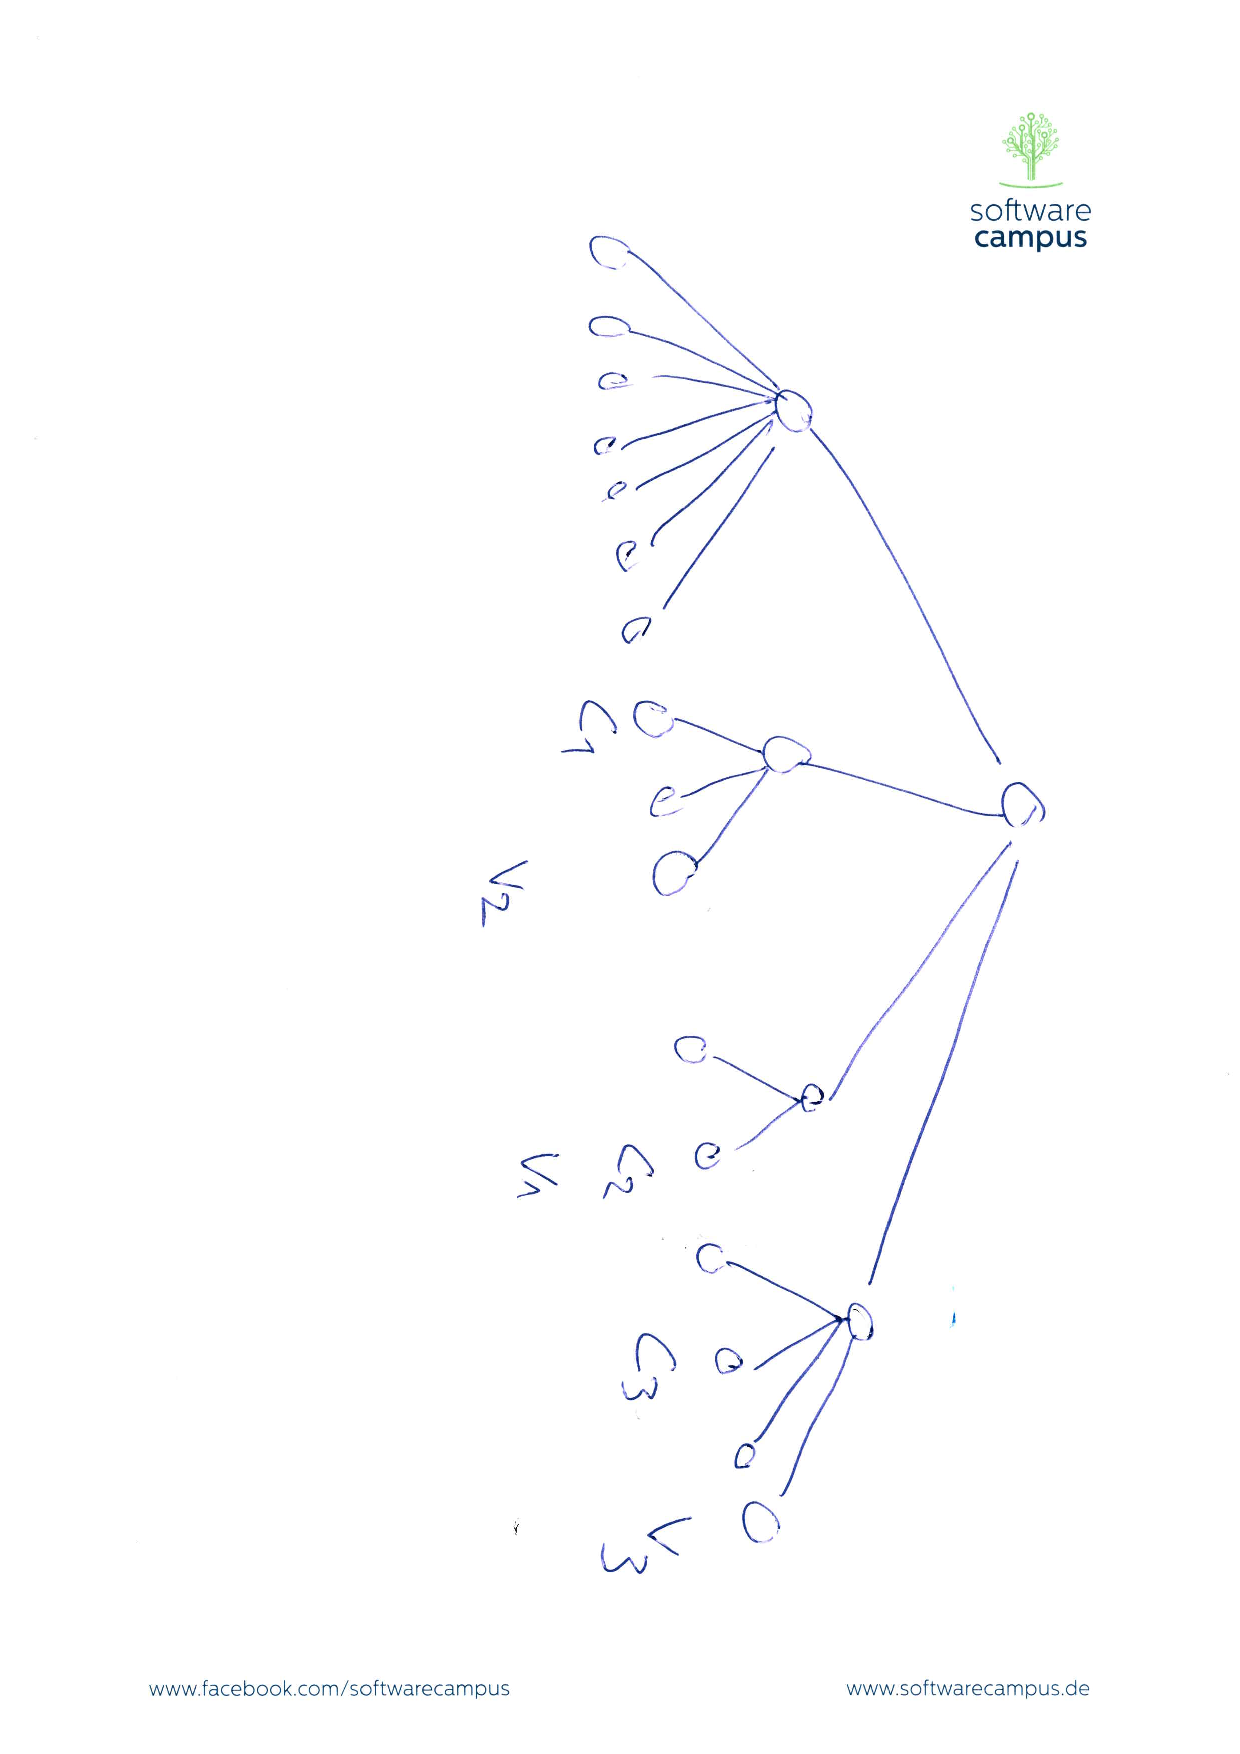
\includegraphics[angle=90,origin=c, height=7cm]{figs/model_fig_skteches/basic_problem}
\caption{basic problem}
\end{figure}
\begin{figure}

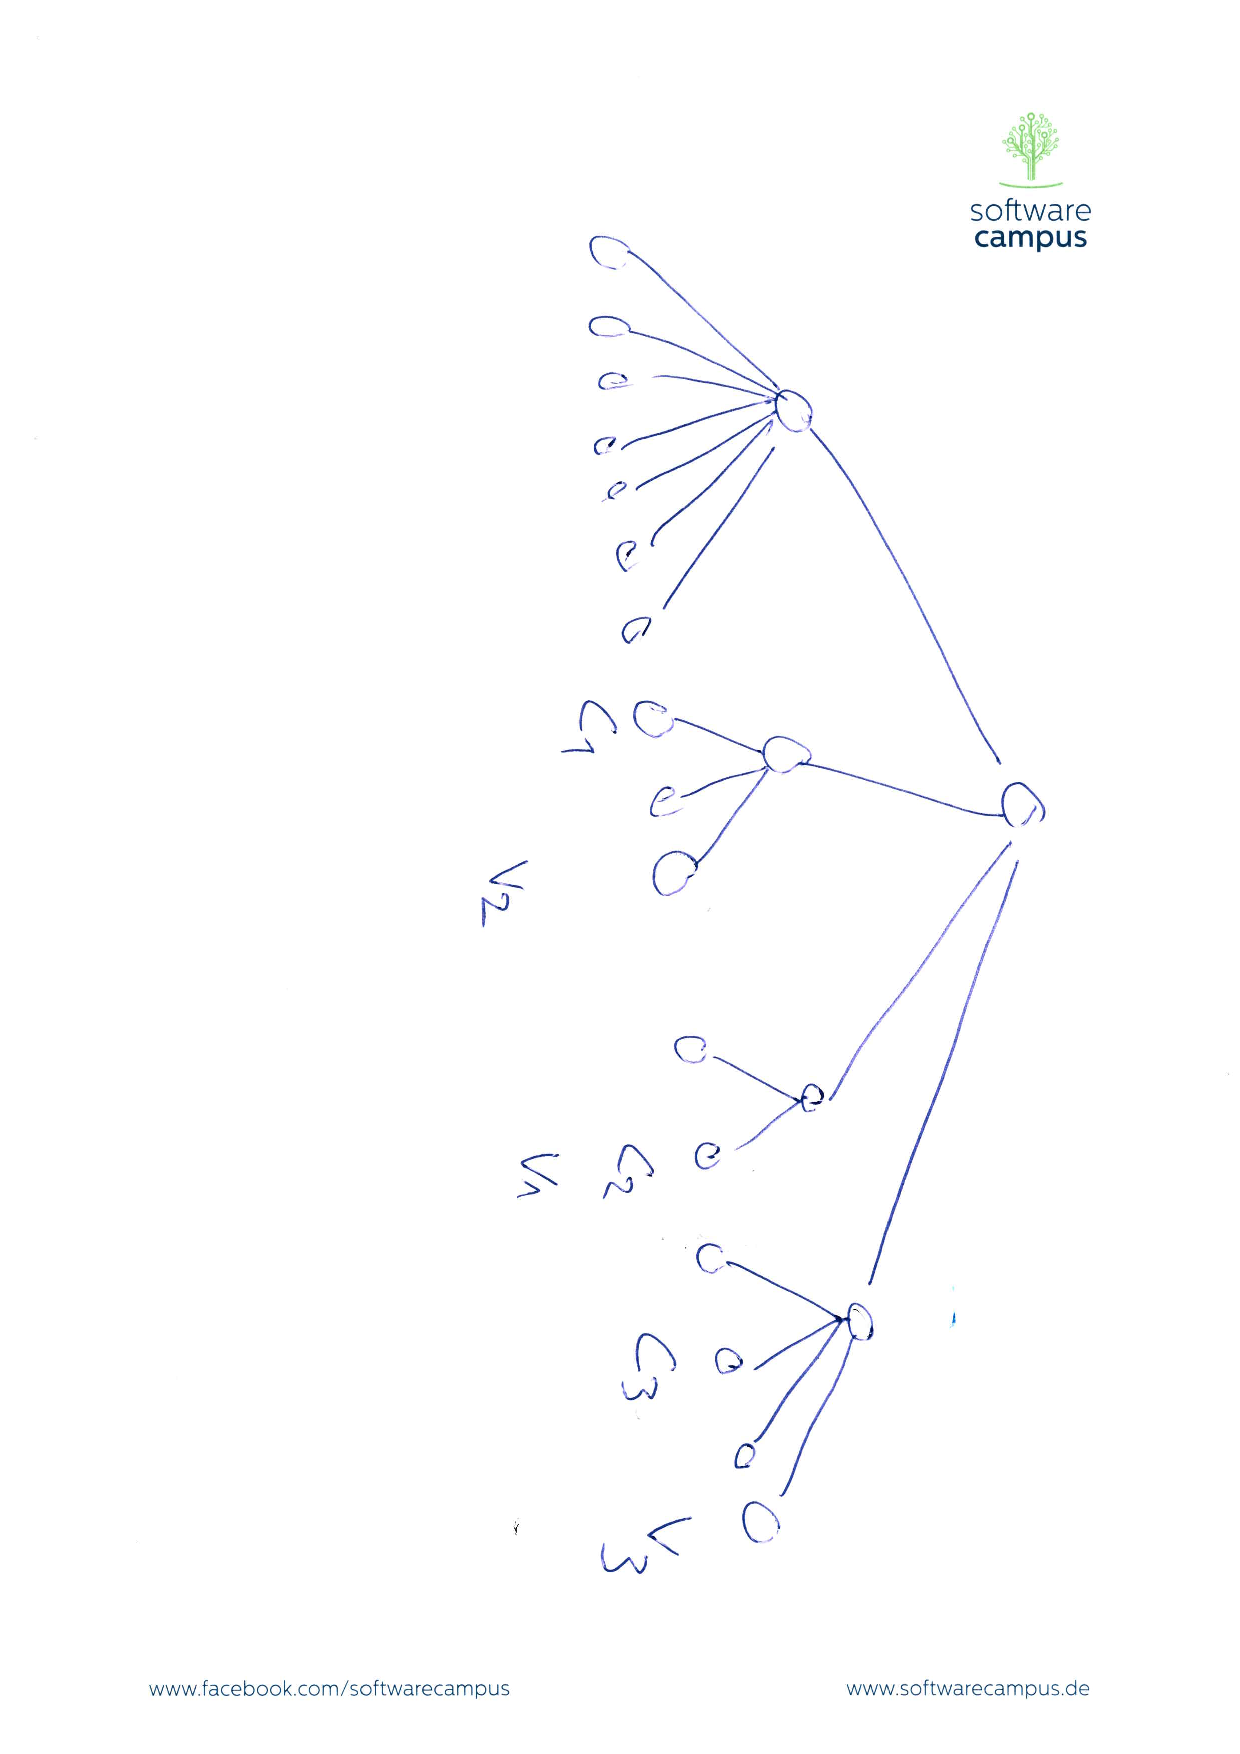
\includegraphics[angle=90,origin=c, height=7cm]{figs/model_fig_skteches/basic_problem}
\caption{solution for basic problem (green is pathes for transfer)}
\end{figure}

Throughout this section we will introduce different properties, to extend this
basic model. These properties can (and will) be combined to form more
challenging instances of $\Problem$.

%\begin{figure}[htbp]
%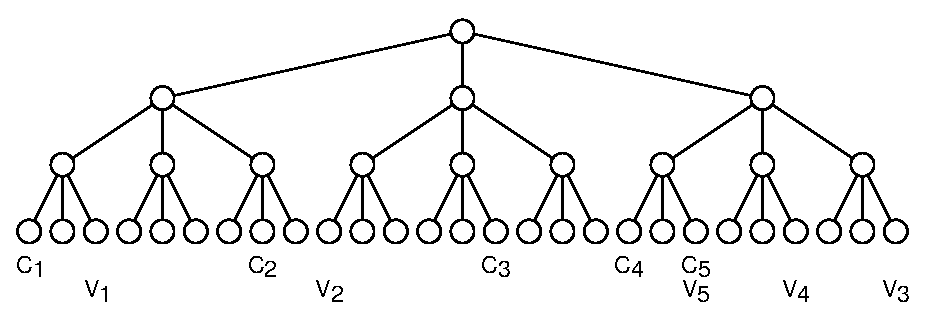
\includegraphics[width = \columnwidth]{figs/basic_scenario_3.eps}
%\caption{An example situation with 5 $\Chunk s$ and $\VM s$. Note that $c_5$
%and $v_5$ are on the same host.}
%\label{fig:model_clean}
%\end{figure}
%
%
%
%Figure~\ref{fig:model_clean} shows an example situation with $n = 5$. The goal
%of the $\Problem$  is to find an assignment of the $\VM s$ to the $\Chunk s$,
%which minimizes the overall bandwidth consumption of the job.
%
%We will now exemplarically examine an assignment of $\Chunk s$ to $\VM s$.
%Assume $c_1$ is assigned to $v_1$, $c2$ to $v2$, $c3$ to $v3$, $c4$ to $v4$
%and $c5$ to $v5$. Since $v_5$ runs on the same host, which contains $c_5$,
%transfering $c_5$ to $v_5$ will consume no bandwidth on the physical links.
%Hence we assume the overall bandwidth costs of the transfer to be $0$. The
%distrance between $v_1$ and $c_1$ is $2$ hops. Hence the transfer of the
%$\Chunk$ to the $\VM$ will consume bandwidth on two links. As a result, the
%overall bandwidth costs is $2 \cdot b_t$, where $b_t$ is the bandwidth
%neccessary for the transfer of a $\Chunk$. $v_4$ is $4$ hops away from $c_4$,
%which results in a total cost of $4 \cdot b_t$. Since the hop distance between
%$v_2$ and $c_2$ is 6, the costs for transferring the $\Chunk$ is $6 \cdot
%b_t$. The same holds for $v_3$ and $c_3$. The overall bandwidth consumption of
%the assignment is hence $18 \cdot b_t$.
%
%This is not an optimal solution for the $\Problem$. To show this, we will
%inspect a similar mapping. The only difference in the optimal mapping, is that
%$v_3$ is assigned to $c_2$ and $v_2$ is assigned to $c_3$. The bandwidth costs
%for transfering $c_2$ to it's assigned $\VM$ do not change, since $v_3$ is
%still $6$ hops away. $c_3$ however is now only $4$ hops away from its assigned
%$\VM$, which results in an overall bandwidth consumption of $16 \cdot b_t$.

\subsection{Communication Costs - $cv$}

\carlo{TODO: new symbol?}

This model extension assumes, that each VM  $\VirtualNode_i \in \VirtualNodes$
has to communicate with each other VM $\VirtualNode_{j \neq i} \in
\VirtualNodes$. Hence, the virtual cluster, which is to be embedded on the
physical substrate no longer consists only of a set of VMs, but is extended by a
set of virtual edges $\VirtualEdges : \VirtualNodes \times \VirtualNodes$.
Similar to the transfer of the chunks to the VMs, these edges have to be mapped
to a path in the host graph, which connects the locations to which the two VMs
are mapped. For the sake of simplicity we assume, that two VMs which communicate
inflict bandwidth cost of $\CostCom$ on each link of the path, which they use
for their communication.

\begin{figure}

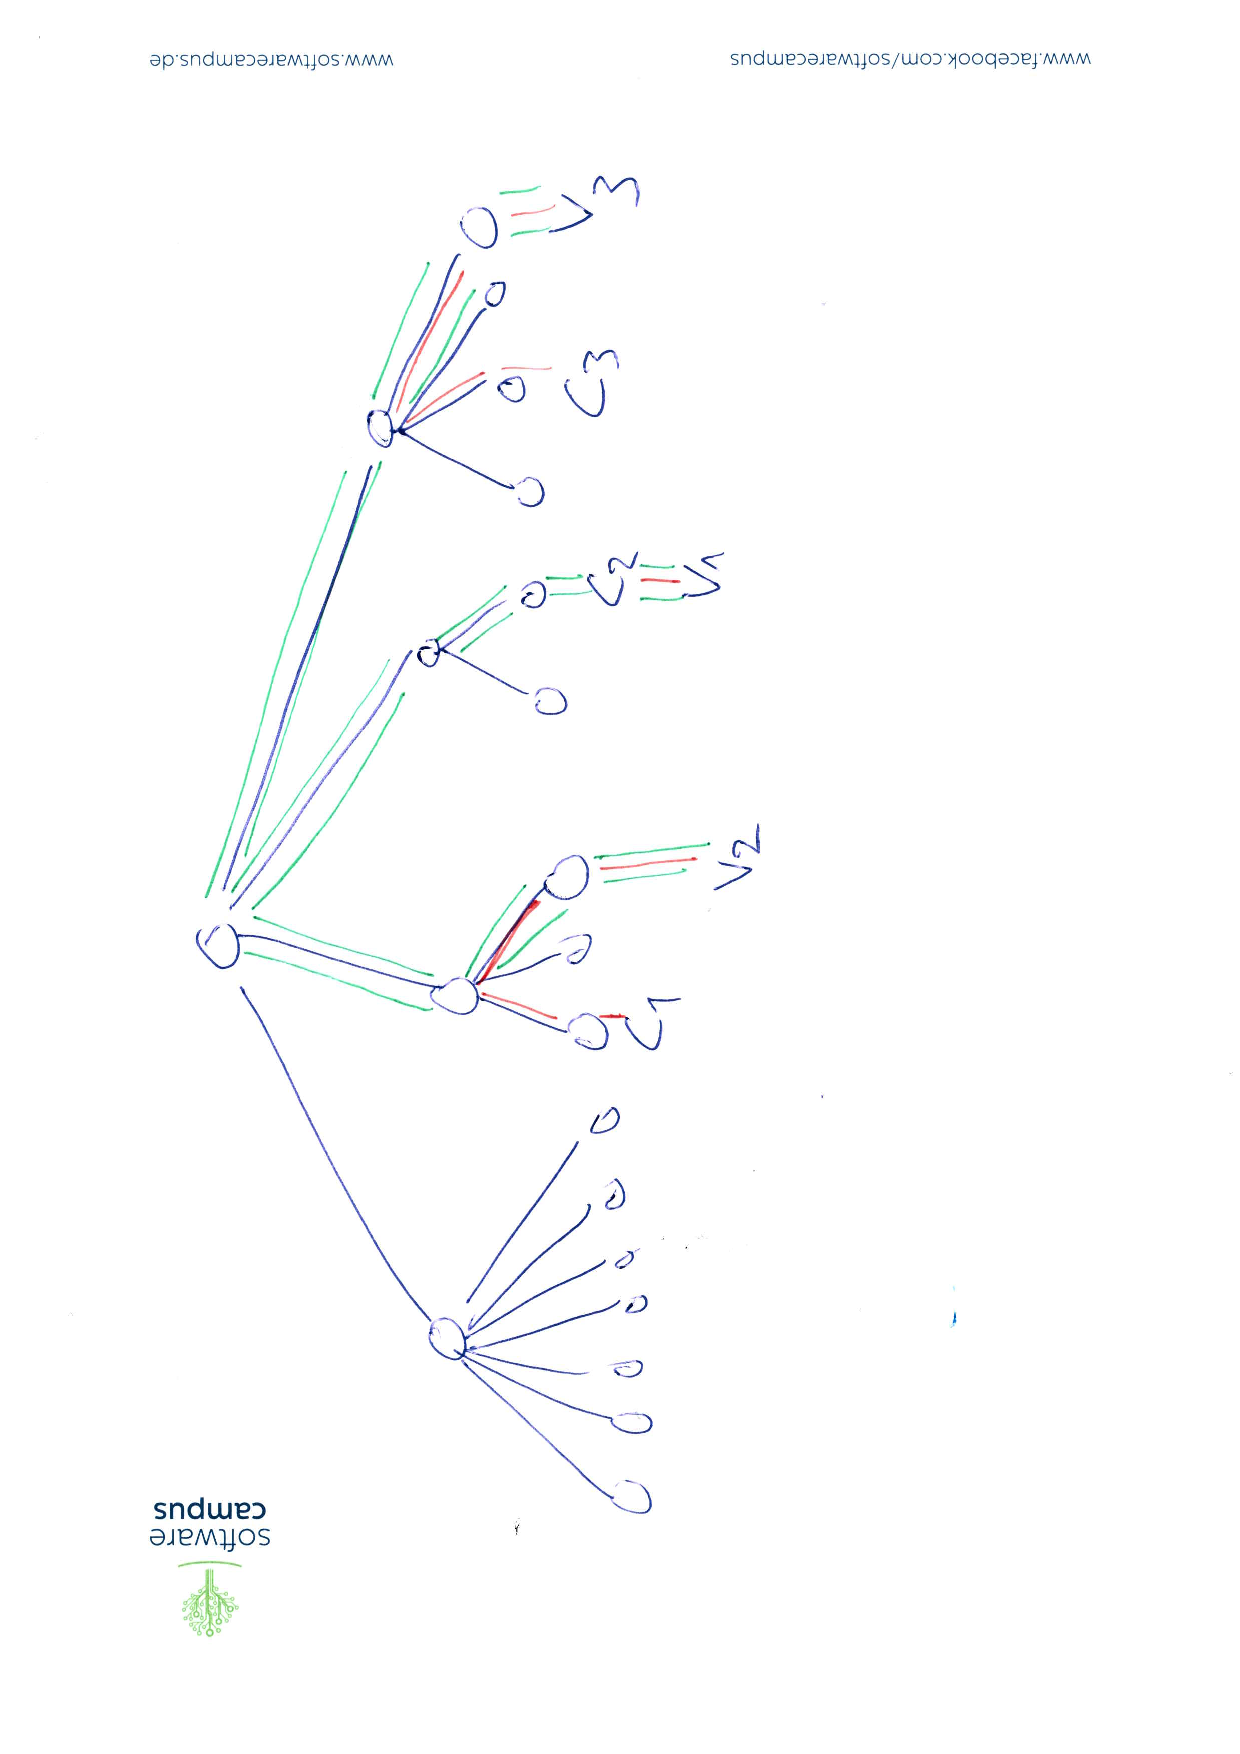
\includegraphics[angle=270,origin=c, height=7cm]{figs/model_fig_skteches/cv}
\caption{solution for problem with cv}
\end{figure}

%So
%far our model accounted bandwidth which is consumed to transfer data from it's
%location in the physical topology to the $\VM$ which will process it. However,
%due to the nature of distributed jobs, the $\VM s$ will also comunicate with
%each other. While we denoted the costs of transfering a chunk over a (1-hop)
%link with $b_t$, we will refer to the bandwidth costs of transfering data
%between a pair of $\VM s$ with $b_c$.


\subsection{Redundant Chunks - $r$}

This property specifies that, instead of having a single chunk $\Chunk_j$, we
have $\RedundancyFactor$ redundant copies of each chunk
$\Chunk_{j_1},\dots,\Chunk_{j_\RedundancyFactor}  \in \Chunks$. These copies are
entirely equal, and only one instance of a specific chunk type (e.g.
$\Chunk_{j_2}$) has to be read by one VM $\VirtualNode_j \in \VirtualNodes$.
Note that we assume chunks to be atomic - they cannot be read from two different
locations, requiering only $\CostTrans / 2$  bandwidth.

\begin{figure}

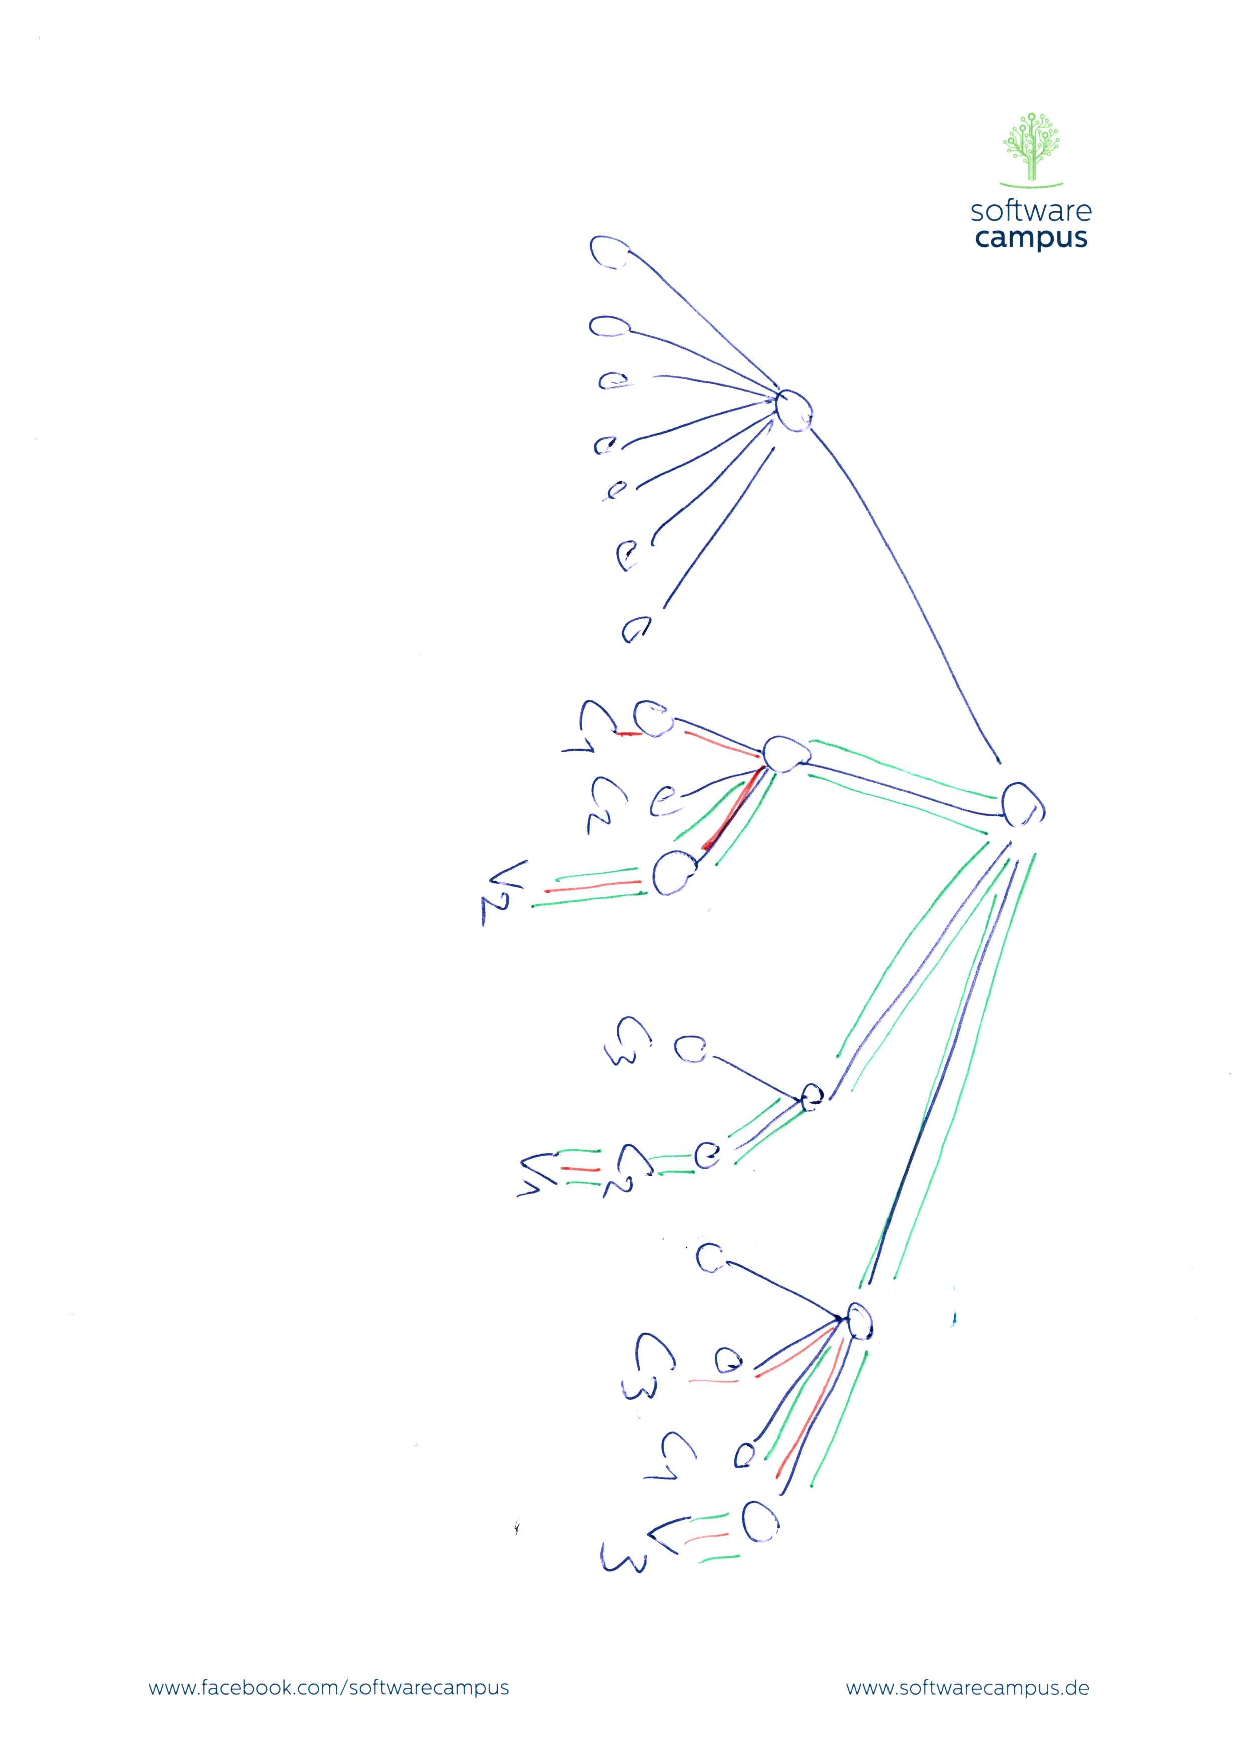
\includegraphics[angle=90,origin=c, height=7cm]{figs/model_fig_skteches/r_cv}
\caption{solution for problem with r}
\end{figure}




\subsection{Multiple Chunks per VM - $ma$}

This extension increases the processing capacities of the VMs. Instead of the
basic 1:1 ratio of VMs and chunks, this extension allows a VM to process
$\MaFactor \in \mathbb{N}^+$ many chunks. We assume, that the data which has to
be transferred to the VM from the chunks cannot be aggregated, and $\Vms =
\ChunkTypes / \MaFactor$.

\begin{figure}

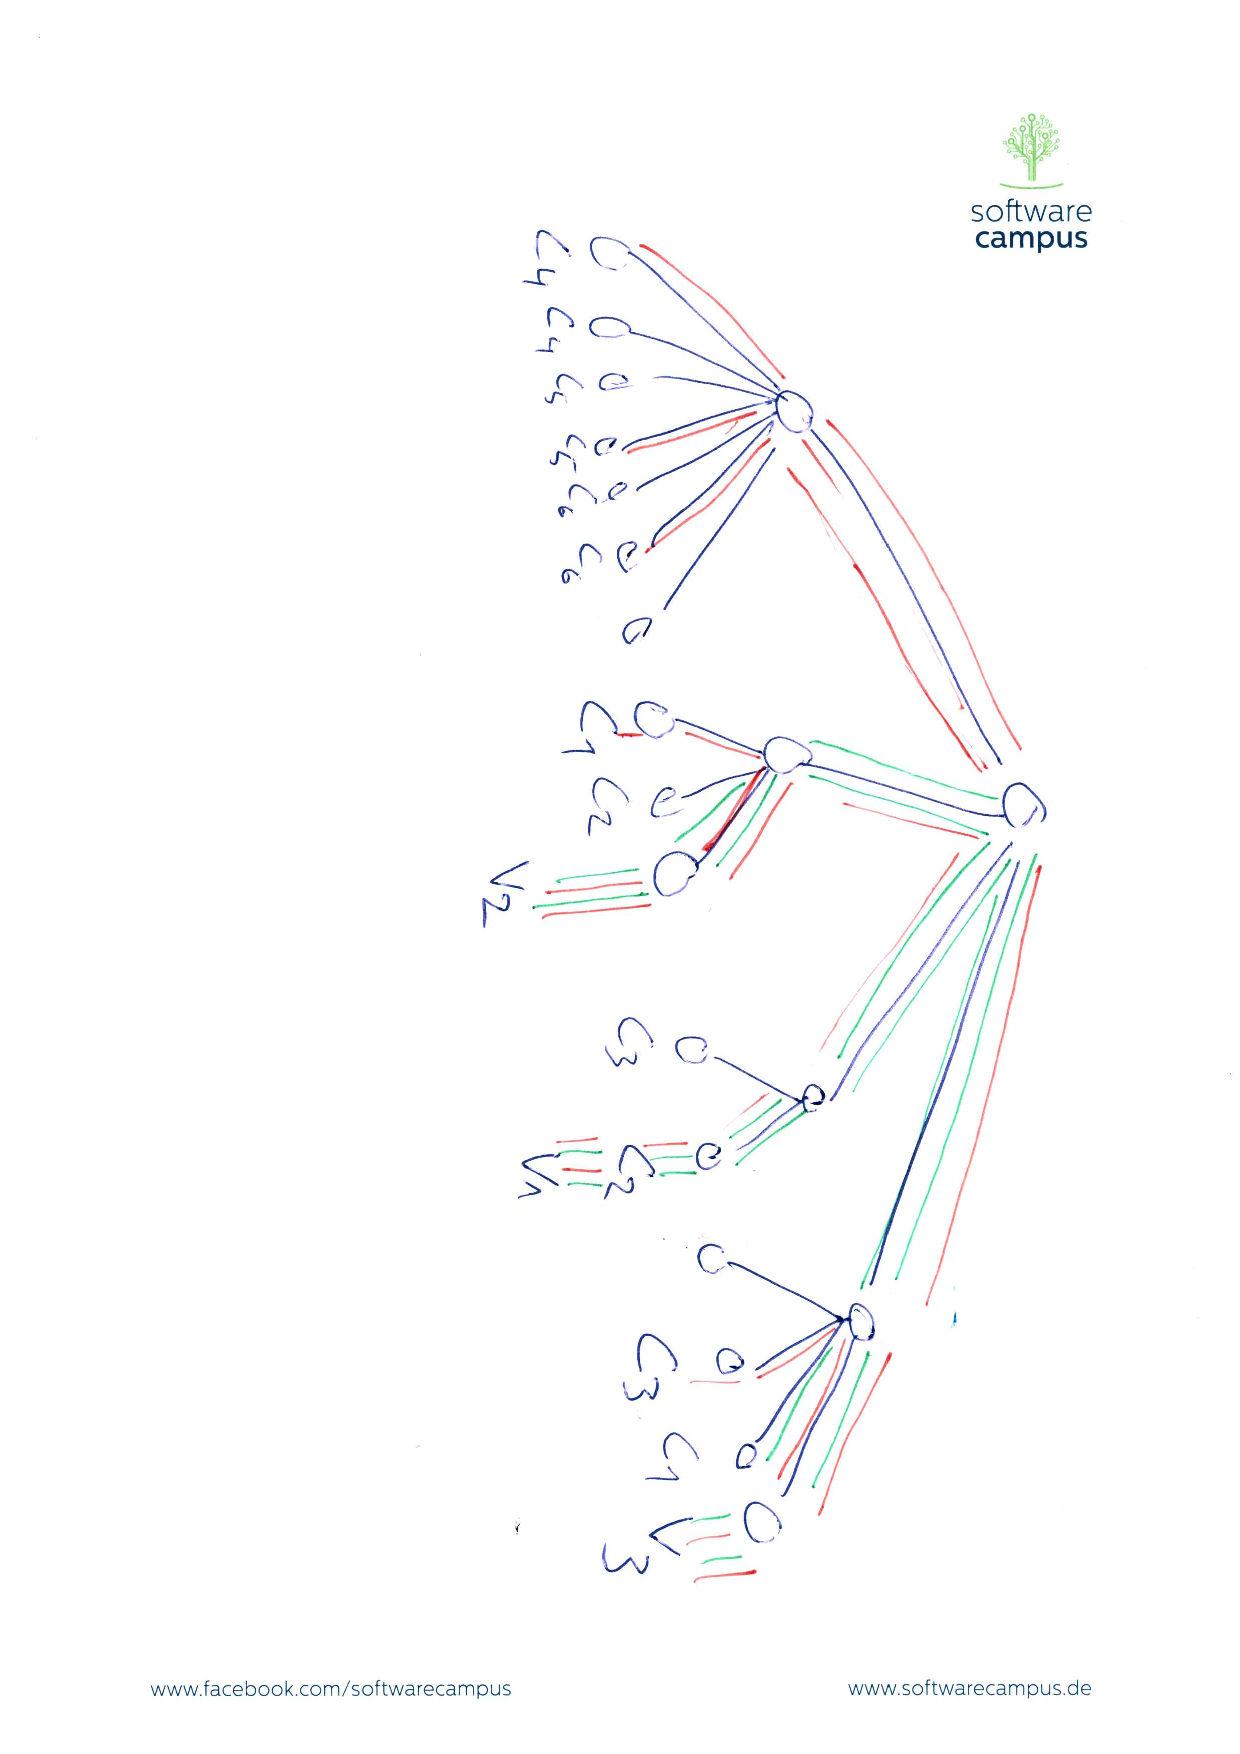
\includegraphics[angle=90,origin=c, height=7cm]{figs/model_fig_skteches/ma_r_cv}
\caption{soltion with ma}
\end{figure}

\subsection{Bandwidth Constraints - $bw$}

So far we only focussed on computing minimal bandwidth costs. However, in
reality the bandwidth which a single link can offer is limited. This model
extension limits the available bandwidth on each link $\SubstrateEdge_i \in
\SubstrateEdges$ in the host graph $\Tree$. We denote the capacity limitations
by $\Capacity : \SubstrateEdges \rightarrow \mathbb{R}$. The sum of all
bandwidth costs on this link, may never exeed it's capacity. Be aware that
this extension introduces infeasible instances.

\begin{figure}

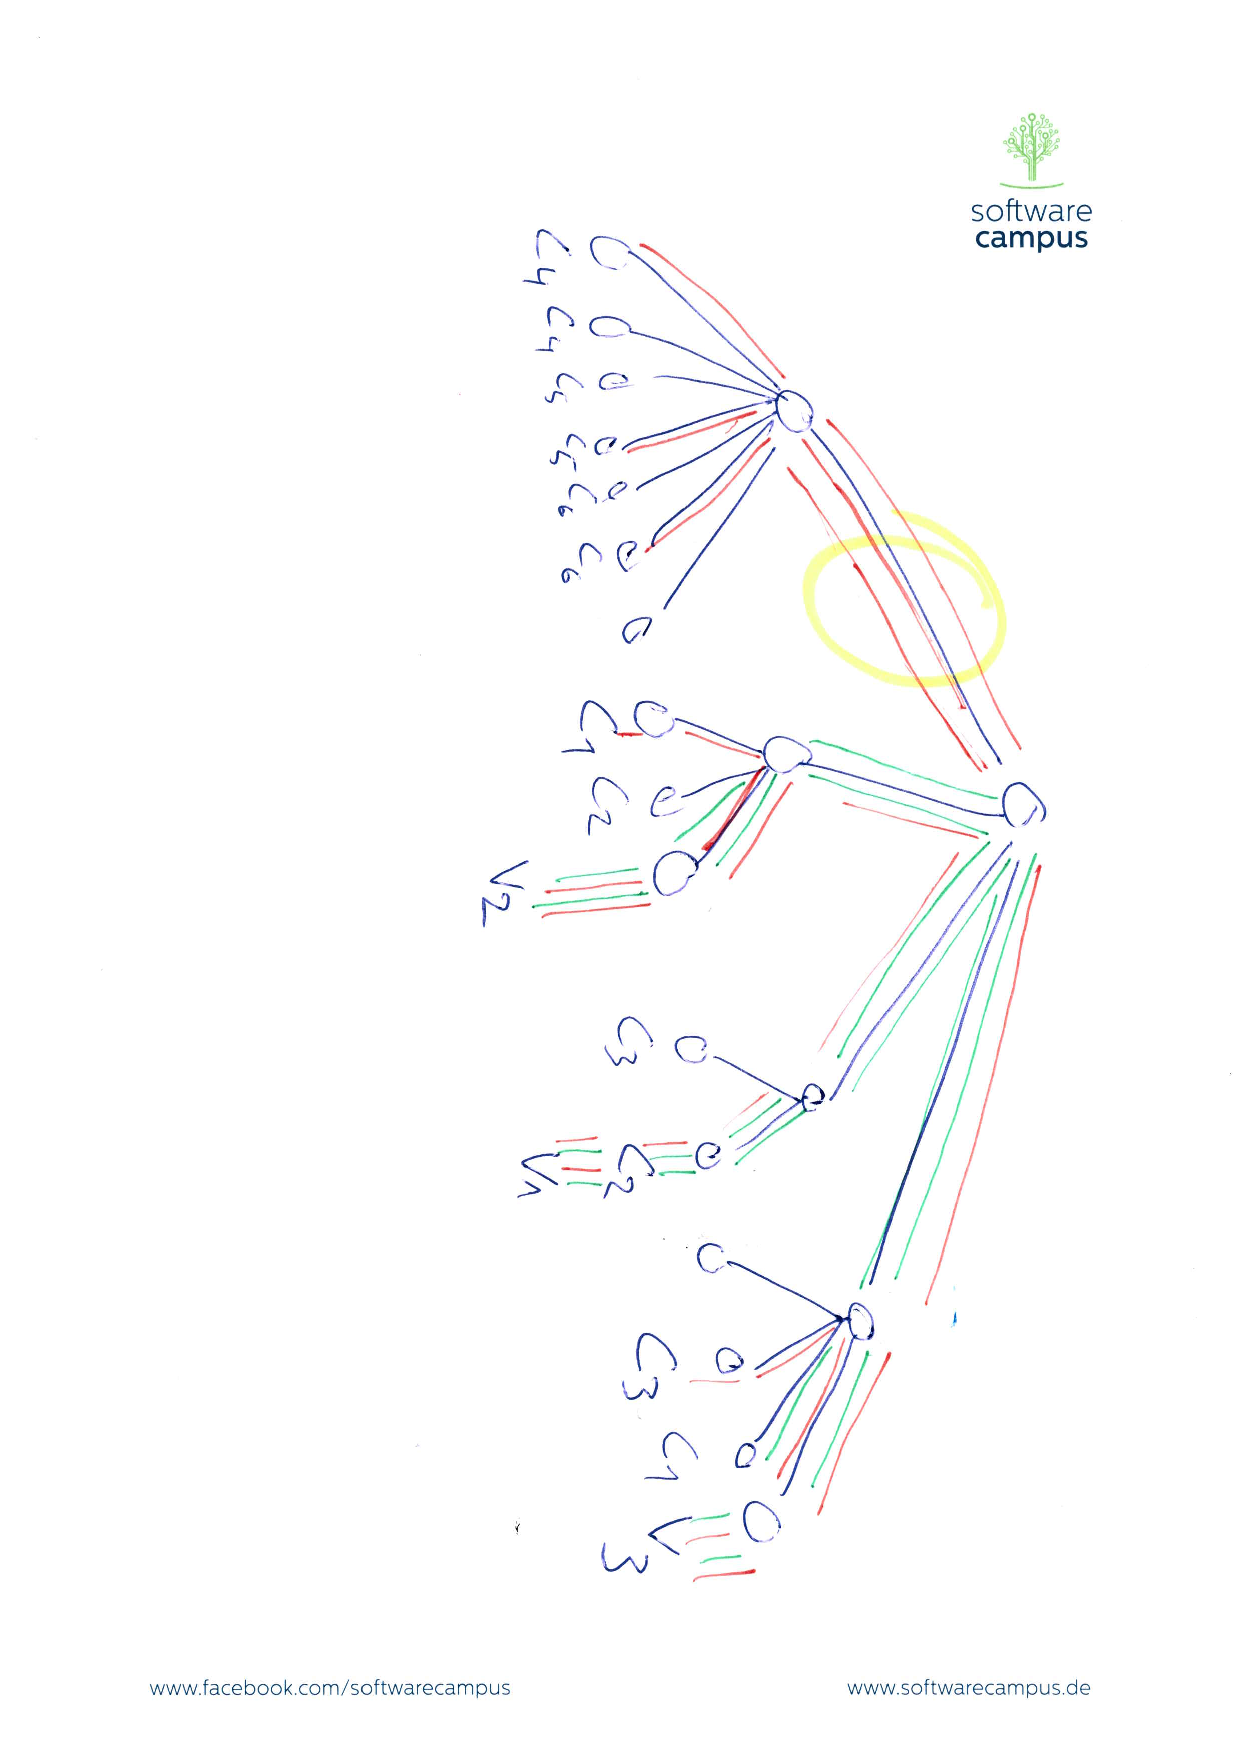
\includegraphics[angle=90,origin=c, height=7cm]{figs/model_fig_skteches/bw_ma_r_cv}
\caption{The bandwidth exceeds the capacity - independent of the chosen assignment}
\end{figure}
\subsection{Free VM Placement - $fp$}

The Free VM Placement property describes a variant of our simple model, where
the positions of the VMs are not given in the problem statement but are
rather chosen by the described strategy. Concretely, $\NodeMapping$ is no
longer given, but part of the optimization within $\Problem$. We assume that
each leaf can only host one VM.


\subsection{Summary of our results}

One day there will be a graph of all problems with arrows
corresponding to reductions and with partitioning to solution
approaches ((M)atching, (D)ynamic, (F)low, (N)p-hard).

\begin{enumerate}
\item basic problem - M
\item ma - M
\item r - M
\item cv - reduces to basic problem
\item bw - F
\item fp - solution of 0 cost
\item ma + r - M
\item  ma + bw - F
\item ma + cv - reduces to ma
\item ma + fp - D
\item r + bw - F
\item r + cv - reduces to r
\item r + fp - solution of 0 cost
\item bw + cv - reduces to bw
\item bw + fp - D
\item fp + cv - D
\item ma + r + bw - F
\item ma + r + cv - reduces to ma + r
\item ma + r + fp - N
\item ma + bw + cv - reduces to ma + bw
\item ma + bw + fp - D
\item ma + fp + cv - D
\item r + bw + cv - reduces to r + bw
\item r + cv + fp - N
\item r + bw + fp - solution of 0 cost
\item bw + cv + fp - D
\item ma + r + bw + cv - reduces to ma + r + bw
\item ma + r + bw + fp - N
\item ma + r + cv + fp - N
\item ma + fp + cv + bw - D
\item r + bw + cv + fp - N
\item ma + r + bw + cv + fp - N
\end{enumerate}


\begin{figure}[htbp]
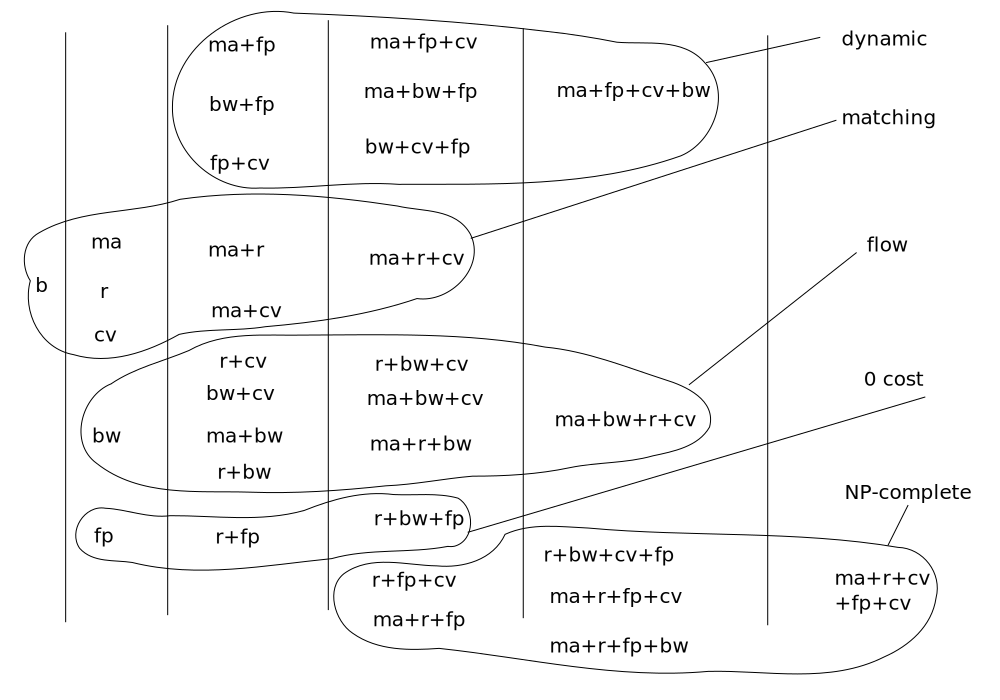
\includegraphics[width = \columnwidth]{figs/summary}
\caption{foo}
\label{fig:summary}
\end{figure}



%%%%%%%%%%%%%%%%%%%%%%%%%%%%%%%%%%%%%
\section{Polynomial-Time Algorithms}\label{sec:poly}

This section gives an overview over model variants which can be solved, and
explains the corresponding algorithms. Figure~\ref{fig:summary} contains an
overview which problems can be solved, and with which algorithms.
\subsection{Matching based solutions} 

In the simplest version of $\Problem$, where all properties are absent, each VM 
is allready placed, the loactions of all chunks are known, and we have to 
compute an assignment of VMs to chunks, such that each VM is assigned to 
exactly one chunk, and each chunk is assigned to exactly one chunk. Hence we 
can transform each instance of $\Problem$ to a minimum weight perfect bipartite 
matching problem. One of the sets is formed by $\VirtualNodes$, the other by the 
set of chunks. A VM has an edge to each chunk. The costs of these edges are 
defined by the hop count between the VM and the chunk in the host graph. Each 
edge which is chosen for the solution of the matching problem, indicates that 
the chunk is assigned to the vm of the edge.

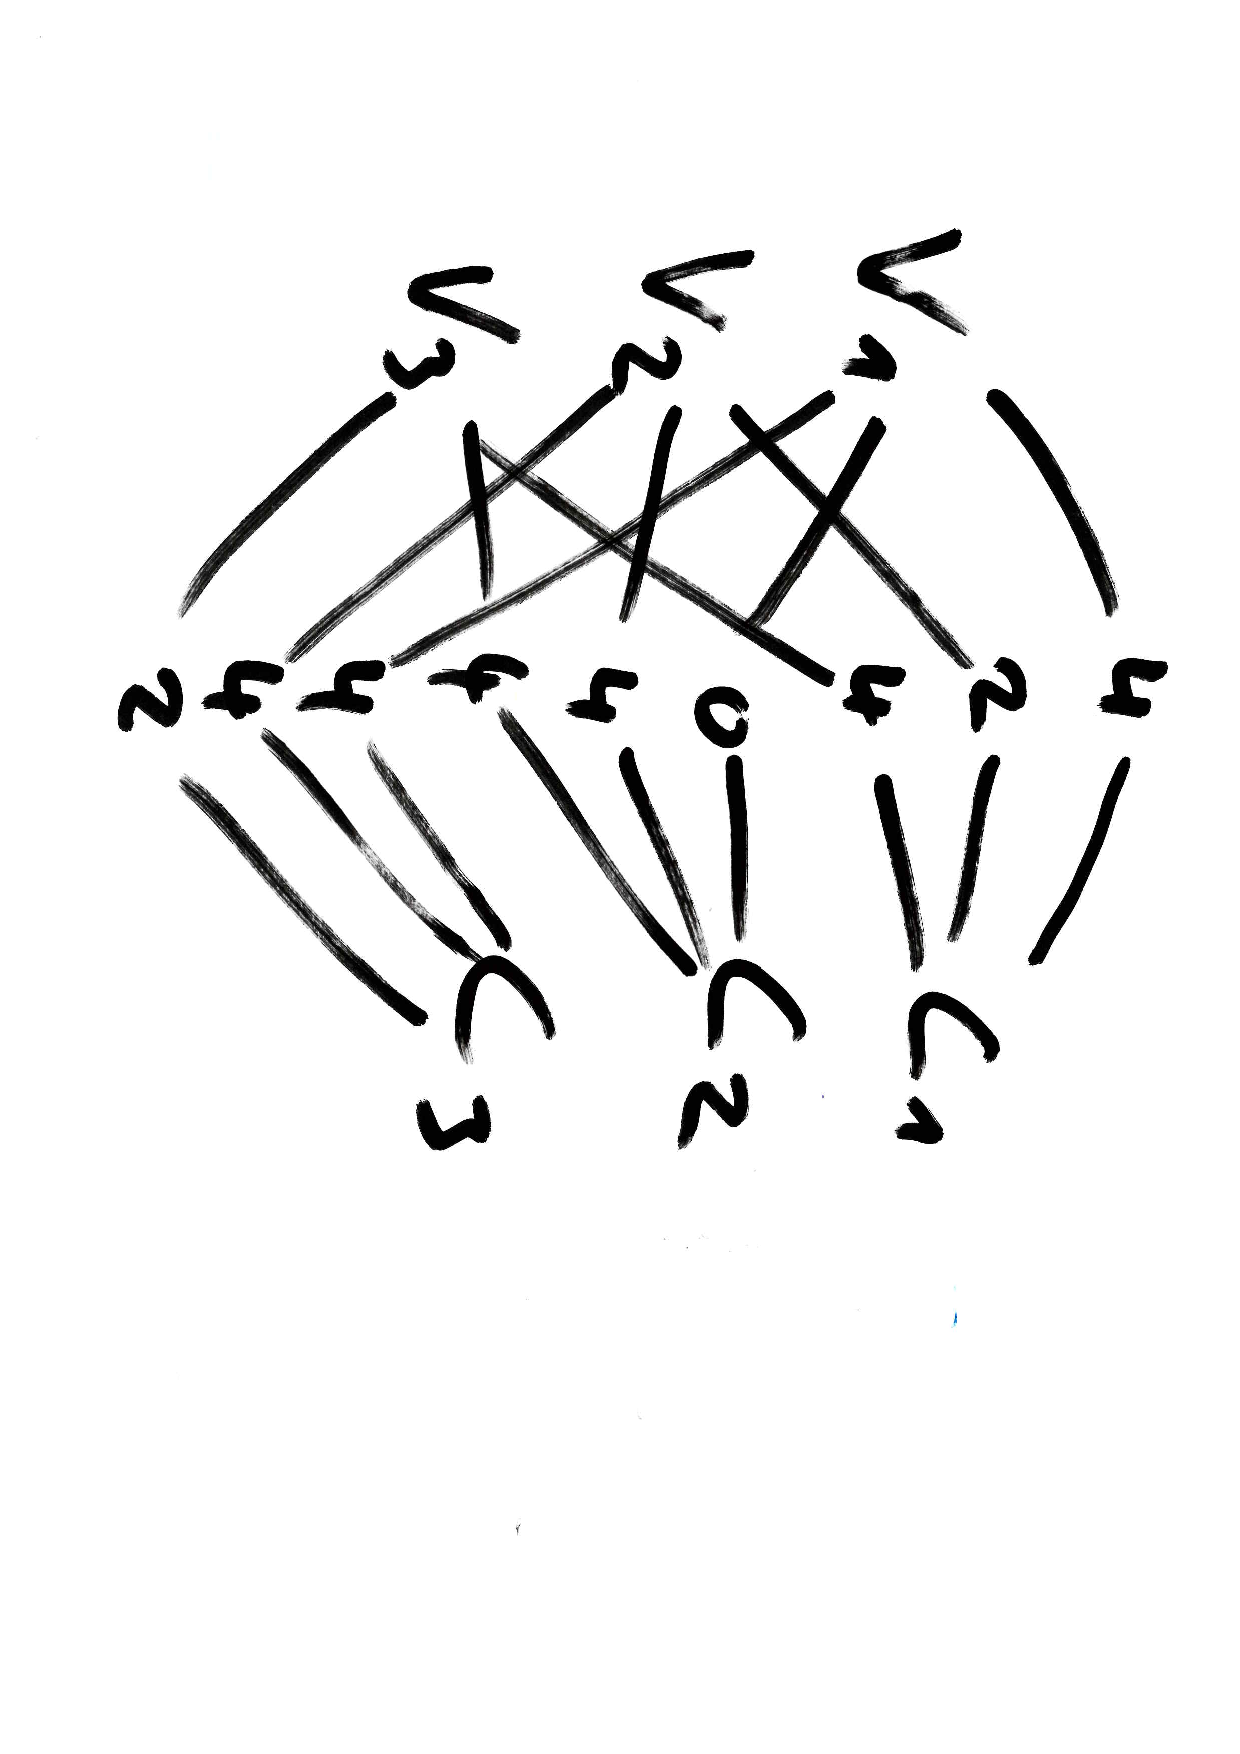
\includegraphics[angle=90,origin=c, 
height=7cm]{figs/model_fig_skteches/matching_basic}

This approach can also be used to solve instance of $\Problem$, which have the 
$ma$ or $r$ property - or even both. 
To Account for the $ma$ property, a single VM has to process exactly 
$\MaFactor$ VMs. Hence we can clone a VM to be represented by $\MaFactor$ Nodes.
In order to incorporate the different 
replicas of the chunks, we depict all copies of a given $\ChunkTypes$ in a 
single %$\ChunkType$ 
node. We connect each VM to all $\ChunkTypes$ using the 
lowest hop count to one of the copies as the weight.

Many algorithms solve the minimum weith perfect matching problem on bipartite 
graphs. The algorithms runtimes depend on  the number of nodes in the 
graph $n$, the number of edges in the graph $m$, and the largest magnitude of 
an edge weight $N$. An efficient algorithm is described by Gabow et al. in 
\cite{gabow_scaling_algorithm} and provides a runtime of $\mathcal{O}(n^{3/4} 
\cdot m \cdot \log n)$ which translates to $\mathcal{O}((\MaFactor \cdot \Vms + 
\ChunkTypes)^{3/4} \cdot  \MaFactor \cdot \Vms \cdot \ChunkTypes \cdot \log 
(2 \cdot h(\Tree)))$, where $h(T)$ denotes the height of the tree.
\subsection{Flow based solutions}

We can solve instances of $\Problem$ where the properties $cv$, $bw$, $r$ and 
$ma$
are present, by reducing it to a series of flow problems on an extended 
host graph. We utilize the following observations:

\newcommand{\Source}{\ensuremath{s}}
\newcommand{\Sink}{\ensuremath{t}}

\begin{enumerate}
\item $cv$ + $bw$ + $r$ + $ma$ degenerates to  $bw$ + $r$ + $ma$. 
The placement of the VMs is given. The bandwdith function $\Capacity$ assigns 
each edge in the host graph $\SubstrateEdge_i$ a capacity 
$\Capacity(\SubstrateEdge_i)$. Since the 
host graph is a tree, there exists only one path between two nodes, and hence 
it is known how much bandwidth has to be allocated on which links, in oder to 
satisfy the communication between the VMs. We can therefore construct a 
problem with $bw$ + $r$ + $ma$ which has the same solutions, by defining 
$\Capacity'(\SubstrateEdge_i)$ as 
$\Capacity(\SubstrateEdge_i) - \textsc{CV}(\SubstrateEdge_i)$, where 
$\textsc{CV}(\SubstrateEdge_i)$ denotes the amount which 
had to be allocated on the link $\SubstrateEdge_i$ for the communication 
between the $\VM s$. If any of the resulting edge capacities is negative, the 
instance of $\Problem$ is infeasible.
\item The required bandwidth $\CostTrans$ between each chosen chunk and the 
assigned VM of a given $\VC$ is 
the same and the pathes to the VMs have to be embedded as unsplittable 
pathes. Hence, all edge capacities in can be normalized to $\CostTrans = 1$.
\item For a (by model) fixed node mapping $\NodeMapping$ and a given chunks to 
vm assignment $\VmChunkAssignment$, the computation of a cost 
optimal link mapping can be transformed to an integral minimal cost multi-commodity 
flow problem, where each VM $\VirtualNode_i$ has a flow demand of $1$ to each 
of its assigned chunks $\VmChunkAssignment(\VirtualNode_i)$. This problem can 
again be transformed into a integral minimum cost single commodity flow problem 
in the following way: 
We introduce a 
super source $\Source$ and edges $\SubstrateEdge_i^+ = (\Source, 
\NodeMapping(\VM_i))$ for 
$i \in \{1,\dots,\Vms\}$ with $\Capacity(\SubstrateEdge_i^+) = \MaFactor$, 
which connects $\Source$ 
to the nodes in the host graph, on which the VMs are located. 
In addition we create a super sink $\Sink$ and edges $\SubstrateEdge_j^- = 
(\VmChunkAssignment(\ChunkLocation(\Chunk_j)), \Sink)$ with capacities 
$\Capacity(\SubstrateEdge_j^-) = 1$, which connect the leaves on which the 
chunks are located to the sink. In this graph we ask for a flow $f$ 
of value $\ChunkTypes$ from $\Source$ to $\Sink$. \carlo{TODO: The 
equivalency...}
\item The replica selection problem can be integrated into the above described 
minimum cost integral single commodity flow problem. Since $\VmChunkAssignment$ 
is not given, but subject to optimization, the edges connecting $\Sink$ to the 
chosen chunks are no longer implementable. Instead, we create a meta node 
$\SubstrateNode_{\Chunk_j}$ for each chunk type 
$\Chunk_j$ and connect it with \carlo{TODO Check directed?!?} edges 
$\SubstrateEdge_{\Chunk_j}^k = (\SubstrateNode_{\Chunk_j}, 
\VmChunkAssignment(\Chunk_{j_k}))$ for all $k \in 
\{1,\dots,\RedundancyFactor\}$. Subsequently we connect the super sink 
$\Sink$ to these meta nodes, via 
edges $\SubstrateEdge_j^- = (\SubstrateNode)$ with 
$\Capacity(\SubstrateEdge_j^-) = 1$. If an integral minimum cost flow $\hat f 
: \SubstrateEdges \rightarrow \mathbb{N}$ of value $\ChunkTypes$ exists, it 
enters the graph at leaves the graph at $\Sink$. Since the only 
edges which connect to $\Sink$ are introduced by our construction $\sum_{j\in 
\{1,\dots,\ChunkTypes\}} \hat f(\SubstrateEdge_j^-) = \ChunkTypes$ holds. From 
$\Capacity(\SubstrateEdge_j^-) = 1$, follows $\hat f(\SubstrateEdge_j^-) = 1 ~ 
\forall j \in \{1,\dots, \ChunkTypes\}$. Hence, for each chunk type $\Chunk_j$, 
$\sum_{k \in \{0,\dots,\RedundancyFactor\}}\hat f(\SubstrateEdge_{c_j}^k) = 1$ 
holds, which - due to the integral solution to the minimal cost flow problem -  
can be interpreted as the replica selection. $\hat f$ enters the graph at 
$\Source$ resulting in $\sum_{i \in \{1,\dots,\Vms\}}\hat f(\SubstrateEdge_i^+) 
= \ChunkTypes = \Vms \cdot \MaFactor$. Due to the capacity limitations this is 
equivalent to $\hat f(\SubstrateEdge_i^+) = \MaFactor ~ \forall i \in 
\{1,\dots, \Vms\}$, which represents $\MaFactor$ outgoing flows for each node 
in the host graph, to which a VM is assigned.
\item To compute $\VmChunkAssignment$ from $\hat f$, we process $\hat f$ in the 
following way: We chose an aribtrary path $\Path = 
\{\SubstrateEdge_{1}, \dots, \SubstrateEdge_{n}\}$, with $\SubstrateEdge_{1} = 
(\Source, \NodeMapping(\VirtualNode_i))$, $\SubstrateEdge_{n} = 
(\SubstrateNode_j, \Sink)$, $\SubstrateEdge_k= (\SubstrateNode_x, 
\SubstrateNode_y) \rightarrow \SubstrateEdge_{k+1} = (\SubstrateNode_y, 
\SubstrateNode_z)$, and $\hat f(\SubstrateEdge)\geq 1 ~ \forall \SubstrateEdge 
\in \Path$. This is a connected path from the source, to the sink, which has 
flow associated on every edge. We set $\VmChunkAssignment(\Chunk_j) = 
\VirtualNode_i$ and reduce $\hat f$ on every edge $\SubstrateEdge \in \Path$ by 
one. This is repeated, until $|\hat f| = 0$. Due to the tree properties of 
$\Tree$, that there is only one path between two nodes, all VM chunk 
assignments generated in this value will have the same overall costs.

\begin{comment}
\item For a given chunk \textit{type} to VM assignment, the replica selection 
problem 
can be integrated into this problem, by introducing nodes 
$\SubstrateNode_\ChunkType$ for each 
chunk type $\ChunkType$ and connect these nodes via edges 
$\SubstrateEdge_\ChunkType = (\SubstrateNode_\ChunkTypes, \SubstrateNode_i)$ 
for all $i$ such that \carlo{Check macieks part for assigned = true}. The 
capacity of all of these edges is set to 
$\Capacity(\SubstrateEdge_\ChunkTypes) = 1$. In this problem 
%
This problem can be converted into 
a integral minimum cost single commodity flow problem, 
%
In addition we create a super sink 
$\Sink$ and edges 
$\SubstrateEdge_\ChunkType^-$ with $\Capacity(\SubstrateEdge_\ChunkType^-) = 1$
%
\item The chunk to vm assignment decision, can be 
integrated into the above described flow problem, by transforming it into a 
integral minimum cost single commodity flow problem.
We introduce a super source $\Source$ and edges $\SubstrateEdge_i^+ = (\Source, 
\NodeMapping(\VM_i))$ for $i \in \{1,\dots,\Vms}$ with 
$\Capacity(\SubstrateEdge_i^+) = \MaFactor$, which 
connects $\Source$ to the nodes in the host graph, to which the VMs are mapped. 
In addition we create a super sink $\Sink$ and edges 
$\SubstrateEdge_\ChunkType^-$ with $\Capacity(\SubstrateEdge_\ChunkType^-) = 1$
%
We extend the flow graph with a nodes $\SubstrateNode_\ChunkType$ for each 
chunk type $\ChunkType$ and connect these nodes via edges 
$\SubstrateEdge_\ChunkType = (\SubstrateNode_\ChunkTypes, \SubstrateNode_i)$ 
for all $i$ such that \carlo{Check macieks part for assigned = true}. The 
capacity of all of these edges is set to 
$\Capacity(\SubstrateEdge_\ChunkTypes) = 1$.
In addition we create a super sink $\Sink$ and edges 
$\SubstrateEdge_\ChunkType^-$ with $\Capacity(\SubstrateEdge_\ChunkType^-) = 
1$, to connect the meta nodes for each chunk type to the super sink.
%Instead of connecting 
%$\Source$ to the nodes, to which the VMs are mapped, we connect $\Source$ to 
%\textit{all leaves} in the host graph via edges $e_\Leaf^+ = (\Source, 
%\SubstrateNode)$. $\Capacity(e_\SubstrateNode^+)$ is set to one, since by 
%the definition of our model, only one VM may be mapped to one server. If a 
%feasible flow $f : \SubstrateEdges \rightarrow \mathbb{N}$ of value $\Vms$ 
%exists, then $\Sum_{\Leaf \in \Leaves}$
\end{comment}
\end{enumerate}




\begin{comment}
\paragraph{FLOW Construction}

This section presents a flow based solution for the variant of the model which 
has bandwidth limitations, communicatin between the $\VM s$ and redundant 
$\Chunk s$.

We start by showing that $cv$ + $bw$ + $r$ is the same problem as $bw$ + $r$. 
The placement of the $\VM s$ is given. The bandwdith function $b$ assigns 
each link in the physical substrate $l_i$ a capacity $c_i$. Since the phyiscal 
stubstrate is a tree there exists only one path between two nodes, and hence it 
is known how much bandwidth has to be allocated on which links, in oder to 
satisfy the communication between the $\VM s$. We can therefore construct a 
problem with $bw$ + $r$ which has the same solutions, by defining $b'(l)$ as 
$b(l) - cv_l$, where $cv_l$ denotes the amount which had to be allocated on the 
link $l$ for the communication between the $\VM s$.

To construct the flow graph, we start from the physical 
substrate. Each edge has a associated costs of $1$ and bandwidth according the 
available bandwidth due to the distribution provided by the $b$ function of the 
$bw$ property of the model. In addition we create and a node for each 
$\ChunkType$. Each of these nodes is connected to every node in the physical 
topology, which has a $\Chunk$ of the corresponding type. The capacity of these 
edges is $1$ and the costs are $0$. In addition we create the source, and 
connect it to all nodes, which represent $\ChunkType s$. The capacity of the 
edges from the sink is $1$ and it's costs are $0$.
On this flow graph, we now solve the (integer) Max-Flow-Min-Cost Problem.

If the resulting maximal flow $\hat f$ has a value $|\hat f|< |C| = |V_V|$, the 
$\Problem$ is infeasible - otherwise we can construct a solution from $\hat f$. 
To construct the solution we choose an arbitrary path $p = \{e_1,\dots, 
e_n\}$ \carlo{TODO check n}, such that $f(e_i) > 1 ~ \forall i \in 
\{1,\dots,n\}$.
\end{comment}

%\subsection{Dynamic programming solution}
Model:
\begin{itemize}
  \item We are given a tree $T$ with capacities $c_e$ on the edges
    (physical network)easured in number of edges)
  \item We are given $n$ chunks that are assigned to leaves of $T$ (at
    most one chunk to one leaf)
  \item Our task is to place $n$ virtual machines on leaves of $T$ (at
    most one virtual machine to one leaf)
  \item Virtual machines can be placed directly on empty leaves or on leaves with chunks
  \item Each chunk has to be transferred to a virtual machine (matching), and the
    cost inlined by that is equal to $b_1$ times distance between
    chunk and virtual machine measured by number of edges
  \item Each virtual machine has to communicate with each other
    virtual machine, and the cost inclined by that is equal to $b_2$
    times distance between each pair of virtual machines meas total cost
\end{itemize}

Let's start by transforming our tree to binary tree with arbitrary
depth. We also introduce weights on edges (either $0$ or $1$). The
strategy we use is to clone every vertex $|children(v)| - 2$ times,
placing subsequent clones as right son of the previous one and placing
subsequent children as left son of the clone. Last child is placed as
right son of last clone.

Let's begin designing our algorithm by writing recursive formula for
minimal cost inclined by placing virtual machines in leaves of a given
tree. Our approach is to evaluate this function using bottom-up
technique using auxilary array, which yields a dynamic programming
solution. To find actual placements of virtual machines in addition to
the cost, we traverse the array backwards, following the path of
minimas.

Keep in mind that number of virtual machines is equal to number of
chunks. However, our function $f$ will be defined by structural
induction on the tree and we will invalidate the property of having
the same number of chunks and virtual machines in a given subtree (which is true when
we look at whole tree).

Let's define $f$ in following way. First argument is a subtree (with
available informations like number of chunks in its leaves), and the
second argument is number of virtual machines that we decided to place
in the subtree (given as first parameter). To calculate optimum
placement of $x$ virtual machines in subtree $T$ ($f(T, x)$) we will
consider every possible split of number $x$ into two positive integer
values: $l$ and $r = x - l$. We will place $l$ virtual machines in
left subtree of $T$ and $r$ virtual machines in right subtree of
$T$. Having such information allow us to compute how much cost we
incline through edge $e_1$ (which connects left subtree of $T$ to root
of $T$) and edge $e_2$ (which connects right subtree of $T$ to root of
$T$). In a given recursive call we charge only those two edges, rest
of edges will be charged is subsequent calls.

Our cost function consists of two factors. First one, communication cost
between virtual machines is easy to compute. We know how many virtual
machines are in left subtree, how many are in right subtree and how
many are in whole tree outside of $T$. For each pair of virtual
machines, first of which is in left subtree and second of which is in
right subtree, we charge $b_2 \cdot (w(e_1) + w(e_2))$. For each pair
of virtual machines, first of which is in left subtree and second of
which is outside $T$, we charge $b_2 \cdot w(e_1)$. Right subtree case
is symmetrical. Second factor of our cost function is the cost of
transferring chunks to virtual machines. Let's call number of chunks
in left subtree as $c_l$ and number of chunks in right subtree as
$c_r$. To incline minimal cost we connect chunks in given subtree to
virtual machines in the same subtree. If we can no longer do that,
because $v_i < c_i (i \in \{l,r\})$, then we connect leftover chunks
to virtual machines in second subtree of $T$. If we can no longer do
that, we connect leftover chunks outside of $T$. This strategy is
optimal, because connecting any other way can be amended (TODO: need
better argument here), inclining lower cost. Connections inside either
left or right subtrees inclines cost $0$ to edges $e_1$ and
$e_2$. Connections between left and right subtree incline cost $b_1
\cdot (w(e_1) + w(e_2))$. Connections from either subtree to outside
of $T$ inclines either $b_1 \cdot w(e_1)$ or $b_2 \cdot
w(e_2)$. Finally, we can write down our formula for $f$:

$$ f(T, x) = min_{l \in \{0, \ldots, x\}} \{ f(T_l, l) + f(T_r, x - l)
+ TransferCost + ConnectionCost\} $$

where $TransferCost$ and $ConnectionCost$ are constants independent of
$l$, and are defined in paragraph above. One simplifying observation
is that to calculate $ConnectionCost$ we can just use the absolute
value of difference
between number of chunks and number of virtual machines in a given
subtree, without knowing which is bigger, because in our model if
there are some virtual machines left, we know that some chunks from
outside will use the same transfer as if we have excessive chunks in
the subtree.

Regarding base case we
trivially define leaf case as having cost $0$ if $x = 0$, cost $b_2
\cdot (n-1) + b_1\cdot n$ if there is no chunk in the leaf, cost $b_2 \cdot (n-1) +
b_1 \cdot (n-1)$ if there is a chunk in the leaf and $\infty$ otherwise.

Capacity constraints are preserved in such way that we put $f(T, x) =
\infty$ if either $e_1$ or $e_2$ transfer cost added to communication
cost exceedes its capacity. Doing so guarantees that this
(impossible) case can never be chosen as a minimum on higher levels of
recurrence calls (unless all other ways are impossible as well). 

When it comes to time complexity of described algorithm, we spend
certain amount of time in every of $2|T|$ vertices of binary
tree (2 is there because of binary transformation). This time can be
bound by iterating over splits of $n$ into two integers, times some
constant and we do it for every possible number of VMs from $0$ to $n$. Therefore, resulting running time is $O(Nn^2)$.



%%%%%%%%%%%%%%%%%%%%%%%%%%%%%%%%%%%%%
\section{NP-Hardness Results}\label{sec:np}

We have seen that even problems with multiple dimensions of
flexibility can be solved in polynomial time. We presented dynamic programming-based solution for
jointly optimization of flexible node placement, assigning multiple
chunks to the same VM, communication among VMs, even under capacity
constraints ($\FP+\MA+\CC+\BW$). We were able to produce solution for optimizing replica selection,
multiple assignment, VM communication, under capacity constraints in
scenario where VMs are already spawned in certain nodes ($\RS+\MA+\CC+\BW$).



This section now points out fundamental
limitations in terms of computational tractability. In particular, we
will show that problems become NP-hard if multiple replicas have to be
assigned to a node ($\FP+\RS+\MA$ is proved NP-hard in
Section~\ref{ssec:fprsma}) or if inter-connects have to be established
($\FP+\RS+\CC$ is proved NP-hard in Section~\ref{ssec:fprscc}); both
results hold even in uncapacitated networks, and even in trees
consisting of two levels only (e.g., in a
datacenter \emph{pod}). Hardness of those problem variants will result
in hardness of 4 other variants -- see generalization graph below.


\begin{figure}[htbp]
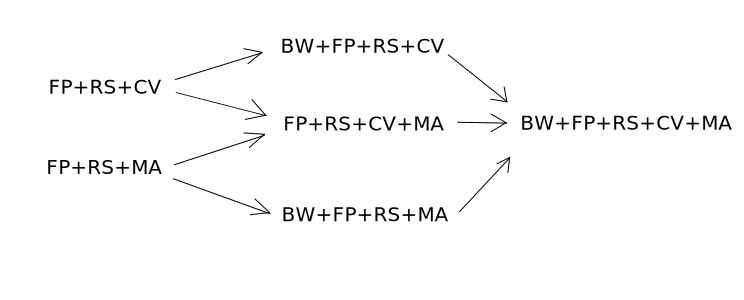
\includegraphics[width = \columnwidth]{figs/np-hierarchy}
\end{figure}



\subsection{Introduction to 3D Perfect Matching}

We start by introducing the NP-complete problem of 3D Perfect Matching
that will serve as problem we reduce from in both proofs. This problem
can be seen as a generalization of bipartite matchings to 3-uniform
hypergraphs, henceforth called $\TDM$.~\cite{3dmatch}

$\TDM$ is defined as follows. We are given three finite and disjoint
sets $X$, $Y$, and $Z$ of cardinality $k$, as well as a subset of triples $T\subset
X \times Y \times Z$.  Set $M \subseteq T$ is a 3-dimensional matching
if and only if, for any two distinct triples $(x_1, y_1, z_1) \in M$
and $(x_2, y_2, z_2) \in M$, it holds that $x_1\neq x_2$, $y_1\neq
y_2$, and $z_1\neq z_2$. Our goal is to decide if we can construct
such $M \subseteq T$ that is perfect, which means that it covers all
elements of $X \times Y \times Z$.

TODO: cite Karp on result of NP-completeness
TODO: image like this: \url{https://upload.wikimedia.org/wikipedia/commons/thumb/5/50/3-dimensional-matching.svg/240px-3-dimensional-matching.svg.png}

\subsection{Multi-Assignments are hard ($\FP+\RS+\MA$)}\label{ssec:fprsma}

Here we will present high-level ideas about encoding $\TDM$ as
 $\FP+\RS+\MA$ instance:

 \begin{itemize} \item For every element of universe $X\cup Y\cup
 Z$, we create chunk type. Processing every chunk corresponds to
 covering whole universe.

 \item We will encode each tripple as $3$ leaves that are close to
 eachother. We place chunk replicas that correspond to elements of the
 tripple.

 \item Placement of VMs will correspond to choice of tripples. No
 matter in which leaf of the gadget the VM will spawn, we will take
 that tripple to solution. VM will process the chunk that it sits on
 top of, as well as chunks in other two leaves of the same gadget.
 
\item We will set threshold cost in such way that no VM process
any chunk outside of the gadget that VM sits in.
\end{itemize}

\textbf{Construction.}
Given an instance $I$ of $\TDM$, we construct an instance $I'$ of
$\FP+\RS+\MA$ as follows:
\begin{itemize}
\item (tree construction) We create a tree consisting of root vertex, and for each tripple
we create a gadget that we attach as direct child of the root. Each
gadget consists of four vertices, one being inner node and three
leaves (see figure below).
\item (chunks and chunk replicas) For each element in $X$, $Y$ and $Z$ we create chunk type
($3 \cdot k$ in total). For each tripple we create $3$ replicas of
chunks that correspond to elements of universe and we place those
replicas in leaves of corresponding gadget
\item (other properties) We set number of VMs to spawn to $k$; we set
$\CostTrans=1$; we set number of slots in each VM to $m=3$; we set
$\Thr=2 \cdot 2 \cdot k$
\end{itemize}

FIXME: The construction is illustrated in Figure~\ref{fig:fprsma}.

\textbf{Correctness.}
We can now show the computational hardness.
\begin{theorem}
$\FP+\RS+\MA$ is NP-hard.
\end{theorem}
\begin{proof}
Let $I$ be an instance of $\TDM$ and let $I'$ be an instance of
$\FP+\RS+\MA$ constructed as described above.
We prove that $I'$ has solution of cost $\leq \Thr$ if ($\Rightarrow$) and only if
($\Leftarrow$)
$I$ has a matching of size $k$.

($\Rightarrow$) Let us take a solution to $\TDM$. We spawn VM in every
gadget that corresponds to chosen triples. We match every chunk in a
gadget to machine in this gadget (only for chosen ones). Solution has
cost exactly $\Thr$.

($\Leftarrow$) Let's take solution to $VC$ instance of cost $\leq \Thr$. We
chose triples that correspond to gadgets where were VMs. Everything
was processed, therefore every element of X,Y and Z is matched.
\end{proof}


\subsection{Inter-connects are hard ($\FP+\RS+\CC$) (reduction from 3D Perfect Matching)}\label{ssec:fprscc}


Next, we prove that the joint optimization of node placement and replica selection
is NP-hard if an inter-connect has to be established between virtual machines.
In our terminology, this is the $\FP+\RS+\CC$ problem.


\textbf{Construction.}
Given an instance of $\TDM$, we construct an instance of a
$\FP+\RS+\CC$ problem as follows. For each element
in the universe $X \cup Y \cup Z$, we construct a chunk; and for each
tripple $T_i$, we construct a gadget that contains
three replicas of chunks corresponding to the elements in the subset (those have 2 hops distance to eachother).
We connect the gadgets to the root, separating nodes from different tripples by 4 hops.

Concretely, let $I$ be an instance of $\TDM$. We will create an instance $I'$
for $\FP+\RS+\CC$ as follows:
\begin{itemize}
\item We set the access cost $\CostTrans$ to a chunk replica to a high value $W$. This will force
nodes to be collocated with the replica.
(For now, we can assume that $W=\infty$; a lower and sufficient bound will be given
in the appendix.)
\item The communication cost in the inter-connect is set to $\CostCom = 1$.
\item The number of nodes (virtual machines) is $\Vms = 3 \cdot k$. TODO: check again
\item We use a threshold $\Thr =  3 \cdot k + 3 \cdot 3 \cdot 2 \cdot (k - 1)$. TODO: check again
\end{itemize}

We construct a height-2 substrate tree
as follows. For each $T_i$ we construct a gadget
consisting of an inner node (a router) and three leaves. Every gadget
contains three chunks, corresponding to the elements of $T_i$.

FIXME: The construction is illustrated in Figure~\ref{fig:fprscc}.

\textbf{Proof of correctness.}
Intuitively, in order to minimize embedding costs,
nodes should be placed on near-by replicas. We use the following
helper lemma.
\begin{lemma}\label{lemma:helper}
In every valid solution $\Sol$ of $I'$ of cost $\leq \Thr$, each gadget
falls in one of two categories:
$k$ gadgets have exactly
$3$ nodes, and $n-k$ gadgets remain empty.
\end{lemma}
\begin{proof}
TODO: use exact cover property here to reason about feasibility

Since $W=\infty$, nodes will always be placed
directly on chunks (the access network cost is zero).
Moreover, since
$\Sol$ is valid, $3 \cdot k$ nodes are mapped
directly to the different chunk locations.
Now, consider any pair of nodes communicating over the
inter-connect; due to our construction, the communication cost
for each such pair is either
2 hops (if they belong to the same gadget) or 4 hops (if they belong
to different gadgets).
The lemma then follows from the observation that $\Thr$
is chosen such that it is never possible to distribute nodes
among more than $k$ gadgets, and that it is always strictly better to
have exactly 0 or 3 nodes per gadget, than any alternative distribution.
\end{proof}

\begin{theorem}
$\FP+\RS+\CC$ is NP-hard.
\end{theorem}
\begin{proof}
Let $I$ be an instance of $\TDM$ and let $I'$ be an instance of
$\FP+\RS+\CC$ constructed as described above.
We prove that $I'$ has solution of cost $\leq \Thr$ if ($\Rightarrow$) and only if
($\Leftarrow$)
$I$ has a solution.

($\Rightarrow$) In order to compute a solution
for $I'$ given a solution for $I$, we proceed as follows.
Given a covering set of tripples $S = \{T_1, T_2, \ldots, T_k\}$, we place three nodes in each gadget that
corresponds to every tripple of $S$. Chunks are matched to VMs that sit on top of them.

The solution has the following cost:
(1) the communication cost inside a gadget is $2 \cdot {3 \choose 2}$,
  as every pair contributes two hops;
  (2) the communication cost from each gadget to all other gadgets is $4
  \cdot 3 \cdot 3 \cdot (k - 1) / 2$, where the factor $2$ is
  for the
  communication over $4$ hops, the factor $3$
  corresponds to the number of nodes per gadget, and
  $3 \cdot (k-1)$ is the number of nodes in remote gadgets;
  as we count each pair twice, we need to divide by two in the end.
Summing up over all $k$ gadgets, we get exactly $\Thr$.

($\Leftarrow$) Given a solution for $I'$,
we can exploit Lemma~\ref{lemma:helper} to construct a solution for $I$.
We know that in any solution of cost at most $\Thr$,
$k$ gadgets contain exactly 3 nodes. These gadgets correspond to a valid
3D Perfect Matching of size $k$: every
chunk and hence element in the $X \cup Y \cup Z$, is matched.
\end{proof}




%%%%%%%%%%%%%%%%%%%%%%%%%%%%%%%%%%%%%
\section{Related Work}\label{sec:relwork}

It is well-known~\cite{talk-about} that the network
can have a significant impact on cloud application
performance, and several solutions have been proposed
over the last years to provide more predictable
network guarantees, such as avoiding multi-tenancy
entirely (see e.g., Amazon's Compute Cluster), by providing relative max-min
per-flow or per-tenant fairness
guarantees~\cite{seawall,netshare,faircloud,elasticswitch}, or by
explicit bandwidth
reservations~\cite{gatekeeper,secondnet,oktopus, proteus, drl}.

Our work focuses on systems with strict performance guarantees,
and there exists a large body of literature
on the general virtual network embedding problem, see~\cite{alloc-survey} for a good survey.
We consider the virtual cluster abstraction proposed
in the Oktopus~\cite{oktopus} paper, and later also studied in
the Proteus~\cite{proteus} paper. However, both papers only present
heuristic algorithms for the virtual cluster embedding problem.
While on average and in our simulations Oktopus~\cite{oktopus} and
Proteus~\cite{proteus} find good embeddings with small footprints,
it is easy to see that the resulting resource footprint
can be arbitrarily bad compared to the optimal solution.
Oktopus can miss solutions where the virtual cluster
is embeddable on a single server, and Proteus can miss efficient embeddings
spanning more than one pod.

FIXME: data locality, matching, etc.

It is well-known~\cite{talk-about} that the network
can have a significant impact on cloud application
performance, and several solutions have been proposed
over the last years to provide more predictable
network guarantees, such as avoiding multi-tenancy
entirely (see e.g., Amazon's Compute Cluster), by providing relative max-min
per-flow or per-tenant fairness
guarantees~\cite{seawall,netshare,faircloud,elasticswitch}, or by
explicit bandwidth
reservations~\cite{gatekeeper,secondnet,oktopus, proteus, drl}.

Our work focuses on systems with strict performance guarantees,
and there exists a large body of literature
on the general virtual network embedding problem, see~\cite{alloc-survey} for a good survey.
We consider the virtual cluster abstraction proposed
in the Oktopus~\cite{oktopus} paper, and later also studied in
the Proteus~\cite{proteus} paper. However, both papers only present
heuristic algorithms for the virtual cluster embedding problem.
While on average and in our simulations Oktopus~\cite{oktopus} and
Proteus~\cite{proteus} find good embeddings with small footprints,
it is easy to see that the resulting resource footprint
can be arbitrarily bad compared to the optimal solution.
Oktopus can miss solutions where the virtual cluster
is embeddable on a single server, and Proteus can miss efficient embeddings
spanning more than one pod.

Finally, we refer the reader to Duffield et al.~\cite{hose-vpn} for an early work
 on \emph{hose}-type specifications in the context of VPN embeddings, and to Gupta et al.~who
 provided and inspired important results also pertaining to hose-based
 virtual cluster embeddings \cite{gupta2001provisioning,Goyal2008}.

%%%%%%%%%%%%%%%%%%%%%%%%%%%%%%%%%%%%%
\section{Conclusion}\label{sec:conclusion}

FIXME

%%%%%%%%%%%%%%%%%%%%%%%%%%%%%%%%%%%%%
\section{Appendix}

%%%%%%%%%%%%%%%%%%%%%%%%%%%%%%%%%%%%%
\bibliographystyle{alpha}
\bibliography{references}

\end{document}
